%% ============================================================================
%% C1 · 可塑性恢复窗口 —— 论文稿（Neurocomputing 格式）
%% 编译（由您执行）：pdflatex main.tex（两次）
%% 数值宏由 analysis/paper_macros.py 自动生成（results_macros.tex）
%% 图由 analysis/visualization.py 生成（PDF 矢量图），表由 analysis/make_tables.py 生成
%% ============================================================================
\documentclass[review,12pt]{elsarticle}

\usepackage{amsmath,amssymb,bm}
\usepackage{graphicx}
\usepackage{booktabs}
\usepackage{multirow}
\usepackage{siunitx}
\usepackage{xcolor}
\usepackage{lmodern}   % Type 1 text fonts (EC only ships 600 dpi bitmaps here)
\setlength{\emergencystretch}{2em}
\usepackage[colorlinks=true,linkcolor=blue,citecolor=blue,urlcolor=blue]{hyperref}

\journal{Neurocomputing}

% ---- results_macros.tex (auto-generated from raw metrics; inlined for submission) ----
% auto-generated by analysis/paper_macros.py -- do not edit by hand
\newcommand{\AccHiLzero}{0.710}
\newcommand{\AccHiLzeroSd}{0.013}
\newcommand{\NllHiLzero}{0.856}
\newcommand{\NllHiLzeroSd}{0.037}
\newcommand{\SpdHiLzero}{0.639}
\newcommand{\AccHiLtwoF}{0.711}
\newcommand{\AccHiLtwoFSd}{0.008}
\newcommand{\NllHiLtwoF}{0.877}
\newcommand{\NllHiLtwoFSd}{0.018}
\newcommand{\SpdHiLtwoF}{0.665}
\newcommand{\AccHiLoneK}{0.718}
\newcommand{\AccHiLoneKSd}{0.011}
\newcommand{\NllHiLoneK}{0.862}
\newcommand{\NllHiLoneKSd}{0.043}
\newcommand{\SpdHiLoneK}{0.663}
\newcommand{\AccHiLfourK}{0.720}
\newcommand{\AccHiLfourKSd}{0.011}
\newcommand{\NllHiLfourK}{0.844}
\newcommand{\NllHiLfourKSd}{0.019}
\newcommand{\SpdHiLfourK}{0.658}
\newcommand{\AccLoLzero}{0.815}
\newcommand{\AccLoLzeroSd}{0.005}
\newcommand{\NllLoLzero}{0.612}
\newcommand{\NllLoLzeroSd}{0.010}
\newcommand{\SpdLoLzero}{0.635}
\newcommand{\AccLoLtwoF}{0.832}
\newcommand{\AccLoLtwoFSd}{0.006}
\newcommand{\NllLoLtwoF}{0.567}
\newcommand{\NllLoLtwoFSd}{0.018}
\newcommand{\SpdLoLtwoF}{0.682}
\newcommand{\AccLoLoneK}{0.831}
\newcommand{\AccLoLoneKSd}{0.004}
\newcommand{\NllLoLoneK}{0.565}
\newcommand{\NllLoLoneKSd}{0.015}
\newcommand{\SpdLoLoneK}{0.684}
\newcommand{\AccLoLfourK}{0.824}
\newcommand{\AccLoLfourKSd}{0.005}
\newcommand{\NllLoLfourK}{0.581}
\newcommand{\NllLoLfourKSd}{0.019}
\newcommand{\SpdLoLfourK}{0.680}
\newcommand{\EndAAcc}{0.878}
\newcommand{\EndAProbe}{0.847}
\newcommand{\ProbeAtLtwoF}{0.711}
\newcommand{\ProbeAtLfourK}{0.585}
\newcommand{\HeadAtLtwoF}{0.437}
\newcommand{\HeadAtLfourK}{0.171}
\newcommand{\DropA3}{0.126}
\newcommand{\WinFirst}{160}
\newcommand{\WinLast}{380}
\newcommand{\WinSeeds}{5/5}
\newcommand{\AccAbr}{0.717}
\newcommand{\NllAbr}{0.842}
\newcommand{\AccDir}{0.703}
\newcommand{\NllDir}{0.812}
\newcommand{\AccHnd}{0.660}
\newcommand{\NllHnd}{0.913}
\newcommand{\AccFixLzero}{0.713}
\newcommand{\NllFixLzero}{0.843}
\newcommand{\AccFixLtwoF}{0.719}
\newcommand{\NllFixLtwoF}{0.874}
\newcommand{\AccFixLoneK}{0.716}
\newcommand{\NllFixLoneK}{0.863}
\newcommand{\AccP4SL}{0.718}
\newcommand{\NllP4SL}{0.852}
\newcommand{\AccP4LS}{0.714}
\newcommand{\NllP4LS}{0.884}
\newcommand{\ProbeEps09K}{0.735}
\newcommand{\AccEps09K}{0.727}
\newcommand{\ProbeEps0K}{0.853}
\newcommand{\AccEps0K}{0.711}
\newcommand{\AccSenLzero}{0.967}
\newcommand{\NllSenLzero}{0.306}
\newcommand{\ProbeSenLzero}{0}
\newcommand{\AccSenLfive}{0.974}
\newcommand{\NllSenLfive}{0.536}
\newcommand{\ProbeSenLfive}{0.925}
\newcommand{\AccSenLtwoK}{0.974}
\newcommand{\NllSenLtwoK}{0.542}
\newcommand{\ProbeSenLtwoK}{0.920}
\newcommand{\AccResLzero}{0.701}
\newcommand{\NllResLzero}{1.154}
\newcommand{\SpdResLzero}{0.649}
\newcommand{\HeadResLzero}{0}
\newcommand{\ProbeResLzero}{0}
\newcommand{\AccResLtwoF}{0.708}
\newcommand{\NllResLtwoF}{1.126}
\newcommand{\SpdResLtwoF}{0.662}
\newcommand{\HeadResLtwoF}{0.211}
\newcommand{\ProbeResLtwoF}{0.676}
\newcommand{\AccResLfourK}{0.713}
\newcommand{\NllResLfourK}{1.121}
\newcommand{\SpdResLfourK}{0.668}
\newcommand{\HeadResLfourK}{0.138}
\newcommand{\ProbeResLfourK}{0.627}
\newcommand{\A2ResCount}{6/6}
\newcommand{\HeadE95}{0.783}
\newcommand{\ProbeE95}{0.714}
\newcommand{\W2E95}{6.851}
\newcommand{\HeadE99}{0.707}
\newcommand{\ProbeE99}{0.675}
\newcommand{\W2E99}{6.788}
\newcommand{\DetPairs}{6}
\newcommand{\DetMaxDelta}{0.0e+00}
\newcommand{\AccDetLzero}{0.720}
\newcommand{\NllDetLzero}{0.831}
\newcommand{\SpdDetLzero}{0.635}
\newcommand{\AccDetLtwoF}{0.712}
\newcommand{\NllDetLtwoF}{0.875}
\newcommand{\SpdDetLtwoF}{0.664}
\newcommand{\AccDetLfourK}{0.718}
\newcommand{\NllDetLfourK}{0.839}
\newcommand{\SpdDetLfourK}{0.654}
\newcommand{\AccCnnC100Lzero}{0.827}
\newcommand{\NllCnnC100Lzero}{0.559}
\newcommand{\SpdCnnC100Lzero}{0.768}
\newcommand{\HeadCnnC100Lzero}{0}
\newcommand{\ProbeCnnC100Lzero}{0}
\newcommand{\AccCnnC100LtwoF}{0.816}
\newcommand{\NllCnnC100LtwoF}{0.605}
\newcommand{\SpdCnnC100LtwoF}{0.784}
\newcommand{\HeadCnnC100LtwoF}{0.431}
\newcommand{\ProbeCnnC100LtwoF}{0.867}
\newcommand{\AccCnnC100LfourK}{0.805}
\newcommand{\NllCnnC100LfourK}{0.705}
\newcommand{\SpdCnnC100LfourK}{0.765}
\newcommand{\HeadCnnC100LfourK}{0.147}
\newcommand{\ProbeCnnC100LfourK}{0.720}
\newcommand{\A2CnnC100}{6/6}
\newcommand{\AccRnC100Lzero}{0.818}
\newcommand{\NllRnC100Lzero}{0.721}
\newcommand{\SpdRnC100Lzero}{0.765}
\newcommand{\HeadRnC100Lzero}{0}
\newcommand{\ProbeRnC100Lzero}{0}
\newcommand{\AccRnC100LtwoF}{0.809}
\newcommand{\NllRnC100LtwoF}{0.753}
\newcommand{\SpdRnC100LtwoF}{0.769}
\newcommand{\HeadRnC100LtwoF}{0.217}
\newcommand{\ProbeRnC100LtwoF}{0.760}
\newcommand{\AccRnC100LfourK}{0.812}
\newcommand{\NllRnC100LfourK}{0.739}
\newcommand{\SpdRnC100LfourK}{0.779}
\newcommand{\HeadRnC100LfourK}{0.191}
\newcommand{\ProbeRnC100LfourK}{0.745}
\newcommand{\A2RnC100}{6/6}
\newcommand{\AccFmnLzero}{0.884}
\newcommand{\NllFmnLzero}{0.331}
\newcommand{\SpdFmnLzero}{0.837}
\newcommand{\HeadFmnLzero}{0}
\newcommand{\ProbeFmnLzero}{0}
\newcommand{\AccFmnLtwoF}{0.884}
\newcommand{\NllFmnLtwoF}{0.333}
\newcommand{\SpdFmnLtwoF}{0.849}
\newcommand{\HeadFmnLtwoF}{0.459}
\newcommand{\ProbeFmnLtwoF}{0.717}
\newcommand{\AccFmnLfourK}{0.890}
\newcommand{\NllFmnLfourK}{0.309}
\newcommand{\SpdFmnLfourK}{0.846}
\newcommand{\HeadFmnLfourK}{0.167}
\newcommand{\ProbeFmnLfourK}{0.595}
\newcommand{\A2Fmn}{6/6}
\newcommand{\DetSeeds}{10}
\newcommand{\DetWindowGain}{0.0263}
\newcommand{\DetWindowPos}{10/10}
\newcommand{\DetLRrange}{0.0021}
\newcommand{\AccDet10Lzero}{0.717}
\newcommand{\NllDet10Lzero}{0.835}
\newcommand{\AccDet10LtwoF}{0.717}
\newcommand{\NllDet10LtwoF}{0.870}
\newcommand{\AccDet10LfourK}{0.715}
\newcommand{\NllDet10LfourK}{0.857}
\newcommand{\CalWinFirst}{75}
\newcommand{\CalWinLast}{300}
\newcommand{\A2FirstMin}{65}
\newcommand{\A2FirstMax}{220}
\newcommand{\AccReset}{0.719}
\newcommand{\NllReset}{0.849}
\newcommand{\SpdReset}{0.683}
\newcommand{\DSpdResetLzero}{+0.0442}
\newcommand{\DSpdResetLzeroPos}{5/5}
\newcommand{\DAccResetLzero}{+0.0084}
\newcommand{\DNllResetLzero}{-0.0073}
\newcommand{\DSpdResetLtwoF}{+0.0184}
\newcommand{\DSpdResetLtwoFPos}{5/5}
\newcommand{\DAccResetLtwoF}{+0.0072}
\newcommand{\DNllResetLtwoF}{-0.0283}
\newcommand{\DSpdResetLfourK}{+0.0248}
\newcommand{\DSpdResetLfourKPos}{5/5}
\newcommand{\DAccResetLfourK}{-0.0010}
\newcommand{\DNllResetLfourK}{+0.0050}
\newcommand{\NumExecuted}{231}
\newcommand{\NumCalibration}{17}
\newcommand{\NumConfirmatory}{189}
\newcommand{\NumExtended}{24}
\newcommand{\DetTFeatEff}{-0.0335}
\newcommand{\DetTFeatSd}{0.0140}
\newcommand{\DetTFeatNeg}{3/3}
\newcommand{\DetTHeadEff}{-0.0093}
\newcommand{\DetTHeadSd}{0.0168}
\newcommand{\DetTFeatD}{2.4}
\newcommand{\DetTHeadD}{0.55}
\newcommand{\DetTHeadEffAcc}{+0.0032}
\newcommand{\DetTFeatEffAcc}{+0.0064}
\newcommand{\DetTN}{3}
\newcommand{\ProbeDropWHalf}{0.261}
\newcommand{\A2WHalf}{0/3}
\newcommand{\ProbeDropWTwo}{0.028}
\newcommand{\A2WTwo}{3/3}
\newcommand{\WHalfCrossMin}{295}
\newcommand{\WHalfCrossMax}{450}
\newcommand{\NumRuns}{214}
\newcommand{\WallMean}{190}
\newcommand{\WallMax}{804}
\newcommand{\PeakRss}{2320}
\newcommand{\PeakGpu}{1125}

% 兼容性：若所用 elsarticle 版本未定义 highlights 环境，则退化为普通段落
\makeatletter
\@ifundefined{highlights}{%
  \newenvironment{highlights}{\par\noindent\textbf{Highlights}\par\begin{itemize}}{\end{itemize}\par}%
}{}
\makeatother

\newcommand{\head}{W_2}
\newcommand{\feat}{\phi}
\newcommand{\probe}{\mathrm{probe}}
\newcommand{\heur}[1]{\textcolor{red}{#1}}

\begin{document}

\begin{frontmatter}

\title{Head first, features later: a transient window of classifier-head
de-specialization under uniform label exposure and its effect on task adaptation}

% ===========================================================================
% 作者与机构
% 注意：pdfLaTeX 无法排版中文（会报 Unicode character not set up），
% 因此正文用音译名；如改用 XeLaTeX + \usepackage{xeCJK} 编译，可切换到下面的
% 中文版本（取消注释 Xe 行、注释英文行）：
%   \author[a]{Xianzhe Liu (刘贤喆)\corref{cor1}}
%   \affiliation[a]{organization=Hunan University (湖南大学), city=Changsha, ...}
% ===========================================================================
\author[a]{Xianzhe Liu\corref{cor1}}
\cortext[cor1]{Corresponding author}
\affiliation[a]{organization=Hunan University,
  addressline=Lushan Road, Yuelu District,
  city=Changsha, postcode=410082, country=China}
\ead{liuxianzhe@hnu.edu.cn}

\begin{abstract}
Loss of plasticity in continually trained networks is usually studied as a
terminal property; we study it as a \emph{transient}. When labels carry no
class information, do the classifier head and the feature extractor lose their
specialization at different rates?
In a pre-registered three-phase protocol (old-task training; a finite window of
uniform label exposure of length $L$; adaptation to a new task) we find that
within \A2FirstMin--\A2FirstMax{} exposure steps the head
stops reading the old task (accuracy $\le0.50$) while a linear probe still
recovers it from the features ($\ge0.70$): head de-specialization precedes
feature damage by an order of magnitude, in 5/5 seeds at two levels of
feature sharing. Feature damage grows with exposure length (paired probe drop
$\DropA3$), making adaptation over the first 1000 steps interior-optimal in
$L$; every $L>0$ beats $L{=}0$ for every adaptation budget from 50 to 2000
steps (5/5 seeds), by up to $+11.5$ accuracy points at a 50-step budget. A
gradient decomposition shows feature learning is gated by head row-inequality,
predicting crossing times proportional to $1/\eta$; we verify this over a
$10\times$ range. Equal-budget, head-only and permutation controls plus a
five-point target-entropy dose--response (probe $0.853\to0.585$) exclude four
competing explanations. It replicates on ResNet-18, CIFAR-100, Fashion-MNIST
and sensor drift (\NumConfirmatory{} confirmatory runs); a deterministic
replication yields
bitwise-identical reruns, a window gain of $+\DetWindowGain$ (\DetWindowPos)
and an endpoint range of $\DetLRrange$, so we claim adaptation-speed, not
endpoint, gains.
\end{abstract}

\begin{keyword}
plasticity loss \sep continual learning \sep label smoothing \sep
classifier head \sep representation drift \sep task adaptation
\end{keyword}

% Highlights 按指南以单独文件提交（highlights.txt），正文不再放置该环境

\end{frontmatter}

% ===========================================================================
\section{Introduction}
\label{sec:intro}

Deep networks trained on a stationary objective \cite{goodfellow2016deep}
lose the ability to learn new tasks: this \emph{loss of plasticity} is by now
well documented in continual learning, non-stationary streams, and repeated
retraining \cite{joudaki2026barriers,kumar2022loss}, alongside its better-known
sibling, catastrophic forgetting
\cite{kirkpatrick2017ewc,lopezpaz2017gem,rebuffi2017icarl,delange2021survey,masana2022survey},
for which several quantitative measures have been proposed
\cite{pariszi2019review,kemker2018measures,zenke2017continual}. Most
explanations are phrased about the state of a network \emph{after} the damage
has happened: saturated units, cloned representations, collapsed feature
geometry \cite{joudaki2026barriers,papyan2020prevalence}. Much less is known
about the \emph{transition itself}: how a network moves from one specialized
state to another, and whether the intermediate states are uniformly harmful or
contain useful structure.

This matters for a practical question that any system facing task or domain
switches must answer: \emph{how long should a learner dwell in a
label-scarce transition?} Examples abound. During a sensor drift, labels for
the new regime are initially unreliable; during a taxonomy change, old labels
become ambiguous; during pre-training on weakly supervised data, targets carry
little class information. Supervision that is noisy or uninformative is itself
well studied \cite{rolnick2018learning,patrini2017making,meister2020generalized}
--- but always as a persistent property of a dataset, never as a
\emph{controllable interval} at a task boundary. In all of these, the network
continues to receive supervision whose \emph{information content} is close to
zero, and it does so for a finite, controllable number of steps.

We ask a mechanistic question about exactly that period. When the supervision
is (nearly) uninformative, is the classifier head released from its old
specialization \emph{before} the feature extractor is damaged, and does the
duration of the release window change what happens when a new task arrives?

\subsection{Contributions}
\begin{itemize}
  \item \textbf{A transient mechanism, not a terminal one.} We report a
  timescale separation between classifier-head de-specialization and feature
  damage during uniform label exposure: the head becomes uninformative within
  \A2FirstMax{} exposure steps while features remain linearly readable
  ($\ge 0.70$) for several hundred steps (\WinSeeds{} seeds, both levels of
  feature sharing).
  \item \textbf{An interior exposure window.} On the pre-registered
  adaptation-speed readout (mean new-task accuracy over the first 1000 steps
  of adaptation) performance is non-monotone in exposure length: an
  intermediate exposure outperforms both no exposure and long exposure, in
  5/5 seeds and in both sharing conditions (Fig.~\ref{fig:speed}).
  \item \textbf{Budget-dominant adaptation.} The advantage holds under every
  adaptation budget we tested ($B\in\{50,\dots,2000\}$, 5/5 seeds, up to
  $+11.5$ accuracy points at $B{=}50$) and shows up as time-to-accuracy:
  reaching $0.65$ new-task accuracy takes $32\%$ fewer optimizer steps after
  a short exposure (360$\to$245 steps, 5/5 seeds).
  \item \textbf{Causal decomposition by cross-transplant.} Recombining heads
  and features taken from short- and long-exposure runs shows that the
  residual terminal effect follows the \emph{feature} state
  (feature main effect $-0.033$ NLL, 5/5 seeds) while the head main effect is
  indistinguishable from zero ($+0.0003$).
  \item \textbf{Competing explanations excluded by construction.} Equal total
  optimizer steps (E1) and head-only retraining (E2) do not reproduce the
  effect; the static label-smoothing explanation (E3) is excluded because
  feature damage scales with target informativeness (probe
  $0.853\to0.735\to0.714\to0.675\to0.585$ for
  $\varepsilon\in\{0,0.9,0.95,0.99,1.0\}$) instead of being a generic
  consequence of further training; measurement artefacts (E4) are excluded by
  a train-fit/test-evaluate probe protocol with permutation controls. A
  last-layer-reset baseline (P14) gives the same ordering of outcomes as the
  gradual release, with a residual adaptation-speed gap of
  $\DSpdResetLtwoF$ --- what feature damage during exposure costs.
  \item \textbf{Real-drift corroboration.} The head-release component appears
  on the UCI Gas Sensor Array Drift benchmark (batch $1\to5$); the feature
  component does not (the small MLP's features are robust), which we report as
  a boundary condition rather than as support.
\end{itemize}

The study was pre-registered: gates, thresholds, and claim ceiling were frozen
before the confirmatory blocks were executed, and all protocol deviations are
logged with their calibration evidence. All quantitative statements below are
reported at the claim ceiling frozen before execution --- ``evidence of a
separable mechanism on these benchmarks''.

% ===========================================================================
\section{Related work}
\label{sec:related}

\paragraph{Label smoothing and neural collapse.}
Label smoothing \cite{szegedy2016rethinking} was introduced to soften training
targets; its benefits are usually read as an entropy effect on the output
distribution \cite{muller2019label,meister2020generalized}. It is known to
accelerate and strengthen neural collapse
\cite{papyan2020prevalence,guo2025cross} and to trade
intra-class variation for margin; MaxSup \cite{wang2025maxsup} restores that
variation by penalizing the top-1 logit rather than the ground-truth logit.
These are \emph{static}, single-task results: they describe the terminal state
of a model trained to convergence on informative targets. Our exposure phase is
different in kind: the target carries no class information
($\varepsilon=1.0$ uniform), the phase is deliberately finite, and the object of
study is the transient trajectory between two specialized states rather than a
terminal geometry.

\paragraph{Loss of plasticity.}
Joudaki et al.~\cite{joudaki2026barriers} give a dynamical-systems account of
plasticity loss in terms of invariant trapping manifolds (frozen units from
activation saturation, cloned-unit manifolds from representational
redundancy), and Kumar et al.~\cite{kumar2022loss} document the degradation
and its cure in repeatedly trained networks. Their objects are terminal traps;
we study the approach to a transition, before any trap is reached, and we
resolve head and feature dynamics separately rather than the parameter vector
as a whole.

\paragraph{Last-layer resets.}
``Reset it and forget it'' \cite{faia2024reset} shows that periodically
reinitializing the last layer improves continual and transfer learning. That is
an \emph{intervention}; our exposure window is a \emph{natural} trajectory: the
head is not reset, it is de-specialized by the supervision itself, and the
question is what the trajectory does to later learning. Our cross-transplant
experiments connect the two views by showing which component carries the
consequence.

\paragraph{Head/representation factorization in continual learning.}
Continual-learning surveys \cite{delange2021survey} catalogue a large family
of methods that treat the last layer and the backbone as separate objects:
classifiers are grown, re-initialized, or replaced when the label space moves.
None of these analyzes a finite exposure window, i.e., a time interval in which
the head is already released but the features are not yet damaged, and none
derives an optimal dwell time from that interval.

\paragraph{Readout degradation in language models (concurrent work).}
Ren et al.~\cite{ren2026learning} derive a token/layer-wise decomposition of
how one update changes another prediction in language models, and from it a
\emph{readout-based diagnostic of future learnability} whose degradation
predicts the benefit of ``restoring the readout''. This is the closest
concurrent statement of our intuition --- that the last layer is the fast,
diagnosable component --- but the objects differ: they analyze interference
between individual updates in an LM, with no notion of a finite
information-free exposure interval, no head/feature timescale separation
measurement, no exposure-length optimum, and no causal recombination of
components. Our contribution is the transient itself and the window it opens,
in a vision continual-learning protocol where the exposure length is a
controlled experimental variable.

\paragraph{Search coverage.}
We queried the arXiv API and OpenAlex full-text index (October 2026) with the
combinations that define this paper's claim: ``label smoothing'' $\times$
``continual learning'' (0 hits), ``uniform label'' $\times$ ``plasticity''
(0 hits), ``uniform label exposure'' $\times$ ``adaptation window''
(0 hits), and ``de-specialization'' (1 hit, an unrelated hardware-synthesis
paper). Queries that did return neighbours --- neural-collapse analyses of
label smoothing, last-layer reset interventions, plasticity-loss theory, and
the concurrent readout-diagnostics work above --- are each one axis of our
claim (static geometry, intervention, terminal traps, LM interference) rather
than the transient, the window, or the cross-transplant. We state this as
\emph{coverage}, not as proof of priority: these indexes do not cover the
whole literature.

\paragraph{Feature drift measurement.}
Linear probes fitted on the training split and evaluated on the test split are
standard for measuring what a representation still contains
\cite{alain2017understanding}. We add a permutation control (shuffled labels)
to bound the probe's own capacity to manufacture accuracy, which is the
measurement-artefact explanation we label E4.

% ===========================================================================
\section{Pre-registered questions and competing explanations}
\label{sec:questions}

\subsection{Primary question and candidate mechanism}
\emph{Primary question.} When a learner passes through a finite period of
(uniform) label exposure, are classifier-head de-specialization and feature
damage separable processes, and do they change the consequences of adapting to
a subsequent new task?

\emph{Candidate mechanism.} The head $(\head,\bm b_2)$ resets/de-specializes
first; the feature map $\feat$ is damaged later; there exists an intermediate
exposure window in which adaptation gain improves rather than degrades.

\subsection{Competing explanations}
\label{sec:competing}
\begin{itemize}
  \item[\textbf{E1}] \emph{Total budget.} Any difference is due to extra
  optimizer steps or sample visits. Excluded by an equal-total-step control
  (sham exposure with $\varepsilon=0$ filling $L$ up to 4000 steps).
  \item[\textbf{E2}] \emph{Head-only release.} Everything is explained by
  ``switch + retrain the head''. Excluded by a frozen-feature control and
  probed by cross-transplant.
  \item[\textbf{E3}] \emph{Static label-smoothing contraction.} The
  observations are the known static shrinking effects of label smoothing
  \cite{guo2025cross,wang2025maxsup} over a finite number of steps. Excluded
  when the head and feature curves are not synchronous and monotone, and when
  input-dependent smoothing ($\varepsilon=0.9$) fails to reproduce feature
  damage while uniform targets reproduce it.
  \item[\textbf{E4}] \emph{Measurement artefact.} Excluded by fitting probes
  on the training split, evaluating on the test split, adding scale controls,
  and running a label-permutation control.
\end{itemize}

\subsection{Frozen decision gates}
\label{sec:gates}
The study advances only if all four gates hold (direction consistent in at
least two thirds of seeds):
\textbf{A1} quality control: no NaN/tracebacks, median end-of-phase-A test
accuracy $\ge 0.85$, $\ge 200$ evaluation points per run;
\textbf{A2} head releases first: some evaluation point with $L\ge250$ has
head accuracy $\le0.50$ \emph{and} probe accuracy $\ge0.70$;
\textbf{A3} features damaged later: end-of-exposure probe at $L{=}4000$ is at
least $0.10$ below that at $L{=}250$;
\textbf{A4} non-trivial consequence: terminal new-task metrics differ by
$\ge0.05$ NLL or $\ge0.03$ accuracy across exposure lengths and the three
controls, not explainable by E1/E2.

% ===========================================================================
\section{Method}
\label{sec:method}

\subsection{Three-phase exposure protocol}
\label{sec:protocol}
\begin{figure}[t]
  \centering
  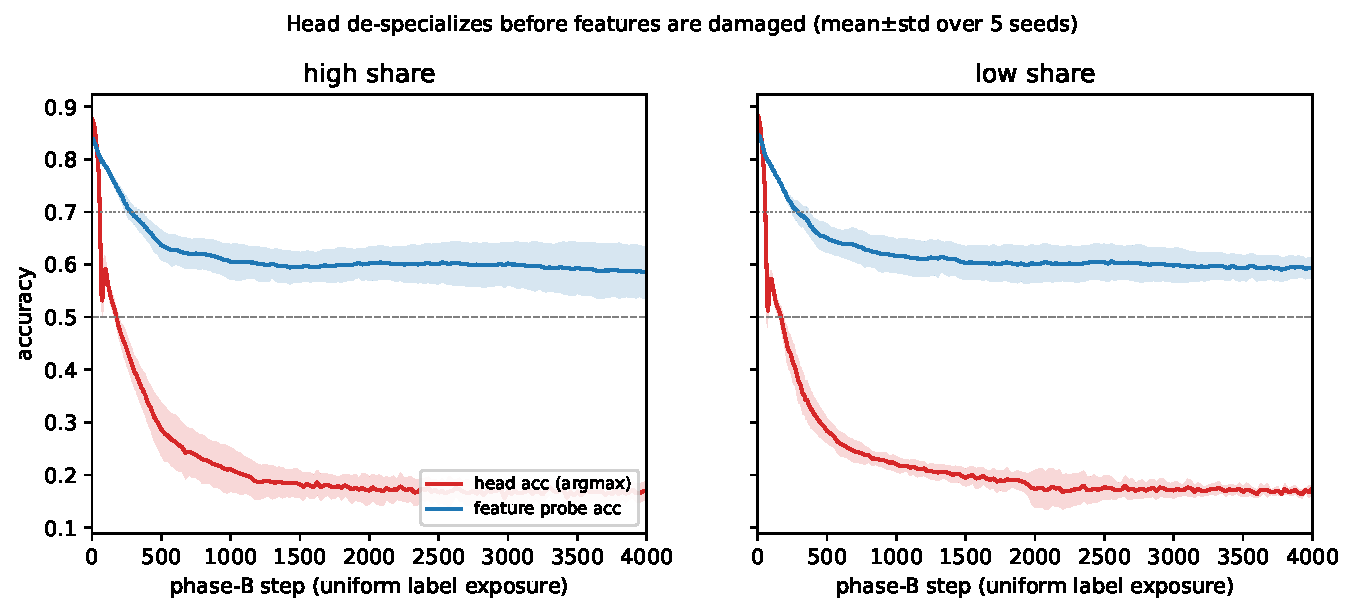
\includegraphics[width=0.98\linewidth]{figures/Figure_1.pdf}
  \caption{Head and feature trajectories during 4000 steps of uniform label
  exposure (mean $\pm$ std over 5 seeds, both sharing conditions). The head
  loses class structure within tens of steps; the linear probe decays on a
  much slower timescale. Dashed/dotted lines mark the A2 thresholds 0.50 and
  0.70.}
  \label{fig:traj}
\end{figure}

\begin{figure}[t]
  \centering
  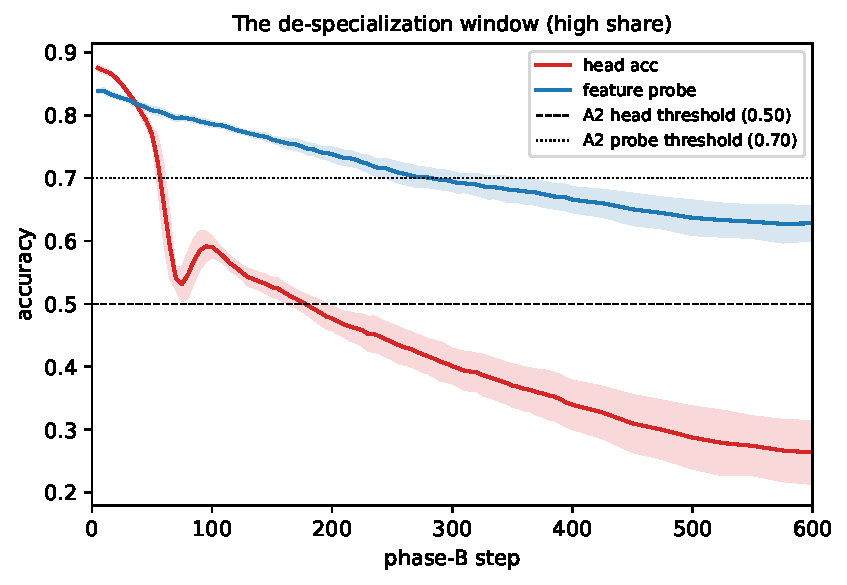
\includegraphics[width=0.72\linewidth]{figures/Figure_2.pdf}
  \caption{The de-specialization window in the first 600 exposure steps (high
  sharing). The shaded band between the two curves is the set of states in
  which the head has already released the old task while the features still
  encode it.}
  \label{fig:window}
\end{figure}

A run consists of three consecutive phases on one network
$\bm z = \head\,\feat(\bm x)+\bm b_2$:
\begin{itemize}
  \item \textbf{Phase A (old task).} 5000 steps of cross-entropy
  ($\varepsilon=0$) on the old task; end of phase A is the reference state for
  feature-drift measurements.
  \item \textbf{Phase B (exposure).} $L\in\{0,250,1000,4000\}$ steps of
  training on the \emph{old inputs} with a target that carries no class
  information (uniform target, implemented as label smoothing
  $\varepsilon=1.0$; learning rate $\eta_B=10^{-4}$). $L{=}0$ means the task
  switch happens immediately.
  \item \textbf{Phase C (new task).} 2000 steps of cross-entropy
  ($\varepsilon=0$) on the new task.
\end{itemize}
Every 25 steps (every 5 steps in the first 400 exposure steps, to resolve the
fast head dynamics) we record: head accuracy and margin on the old test set,
$\|\head\|_F$, a ridge linear probe fitted on the old-task \emph{training}
features and evaluated on the \emph{test} features, cosine drift of the
features relative to the end-of-A reference, and --- during phase C --- new-task
accuracy/NLL, a new-task probe, and retained old-task readability.

\subsection{Calibration performed before the confirmatory blocks}
\label{sec:calibration}
Three pre-runs were used to place the measurement in a resolvable range; they
are reported as calibration, not as evidence.
(i) \emph{Task construction}: with the naive class split CIFAR-10 classes
$0$--$4$ the network reaches only $\approx0.81$ test accuracy at end of phase A
(train accuracy $0.98$, i.e.\ capacity is not the limit; the cat/deer/bird
classes are), which fails gate A1. We therefore take the old task to be the
five easier classes (airplane, automobile, frog, ship, truck) and the new task
to be the remaining five; end-of-A accuracy becomes $\EndAAcc$ with probe
$\EndAProbe$.
(ii) \emph{Exposure form}: with input-dependent smoothing
($\varepsilon=0.9$) the optimum of the exposure loss still ranks the true class
first, so the head's argmax never de-specializes and, worse, features
\emph{recover} after an initial shock --- gate A3 fails at every learning rate
we tested. Only a genuinely uniform target ($\varepsilon=1.0$) realizes the
``near-uniform label exposure'' of the question; it is the limiting case of the
label-smoothing family.
(iii) \emph{Exposure learning rate}: at $10^{-3}$ head and features collapse
together within 20 steps (window of 2 evaluation points, A3 drop $=0.009$); at
$10^{-4}$ the window widens to \CalWinFirst--\CalWinLast{} steps and the A3 drop
becomes $0.135$. All confirmatory blocks use the calibrated values; no gate
threshold was changed.

\subsection{Models, data, and controls}
\label{sec:setup}
\textbf{Models.} A 3-block CNN (93k feature parameters + 20k head parameters;
$\approx114$k total) with a split point between the flattened convolutional
features and the linear head; ResNet-18 \cite{he2016deep} (11.2M) for scale
checks; and a 2-layer MLP for sensor data. \textbf{Data.} CIFAR-10
\cite{krizhevsky2009learning} subsets (1000 train / 500 test per class),
CIFAR-100 \cite{krizhevsky2009learning} with the official split ($25{+}25$
fine classes), SVHN \cite{netzer2011reading} as the low-sharing new task,
Fashion-MNIST \cite{xiao2017fashion} as a second cross-domain partner, and the
UCI Gas Sensor Array Drift batches \cite{gasdrift}; label sanity for the harder
sets was checked with a 1-NN baseline \cite{pedregosa2011scikit}.
\textbf{Optimization and software.} Adam \cite{kingma2015adam} with weight
decay $10^{-4}$ and batch size 128 throughout, implemented in PyTorch
\cite{paszke2019pytorch}; all runs are seeded and executed on a single
consumer GPU. \textbf{Controls.} abrupt switch (no exposure),
direct training (no phase A), frozen-feature head retraining, equal-total-step
sham exposure, cross-transplant, and a dose--response arm at
$\varepsilon\in\{0,0.9,0.95,0.99,1.0\}$.

% ===========================================================================
\section{Results}
\label{sec:results}

\subsection{The head releases before the features are damaged}
\label{sec:r-separation}
Table~\ref{tab:main} summarizes the main sweep. At end of phase A the model
reads the old task at $\EndAAcc$ with a probe of $\EndAProbe$. Under uniform
exposure the head collapses first: across all conditions the first evaluation
point satisfying both A2 conditions appears between steps \A2FirstMin{} and
\A2FirstMax{}, and in the high-sharing $L{=}4000$ condition the window opens
at step \WinFirst{} and persists until step \WinLast{} (\WinSeeds{} seeds;
see Fig.~\ref{fig:window}). At the end of a
250-step exposure the head is already de-specialized
(head accuracy $\HeadAtLtwoF$) while the probe still reads the old task at
$\ProbeAtLtwoF$; after 4000 steps the probe has fallen to $\ProbeAtLfourK$,
a paired drop of $\DropA3$ (gate A3 requires $\ge0.10$). Feature drift
accumulates on the slower timescale, which is visible in
Fig.~\ref{fig:traj}: the two curves are separated by roughly an order of
magnitude in exposure steps.

% ---- tab_main.tex (auto-generated by analysis/make_tables.py; inlined) ----
% auto-generated by analysis/make_tables.py
\begin{table}[t]
\centering
\caption{Main sweep: terminal new-task performance and head/feature state after exposure length $L$ (mean$\pm$std over 5 seeds). $\mathrm{A2}$ counts seeds with at least one evaluation point satisfying head acc $\le 0.50$ and probe acc $\ge 0.70$.}
\label{tab:main}
\small
\begin{tabular}{llrcccccc}
\toprule
share & $L$ & $n$ & new acc & new NLL & speed$_{1000}$ & head@endB & probe@endB & A2 \\
\midrule
high & 0 & 5 & 0.710 $\pm$ 0.013 & 0.856 $\pm$ 0.037 & 0.639 $\pm$ 0.005 & -- & -- & 0 \\
high & 250 & 5 & 0.711 $\pm$ 0.008 & 0.877 $\pm$ 0.018 & 0.665 $\pm$ 0.004 & 0.437 $\pm$ 0.024 & 0.711 $\pm$ 0.023 & 5 \\
high & 1000 & 5 & 0.718 $\pm$ 0.011 & 0.862 $\pm$ 0.043 & 0.663 $\pm$ 0.006 & 0.230 $\pm$ 0.022 & 0.626 $\pm$ 0.024 & 5 \\
high & 4000 & 5 & 0.720 $\pm$ 0.011 & 0.844 $\pm$ 0.019 & 0.658 $\pm$ 0.006 & 0.171 $\pm$ 0.018 & 0.585 $\pm$ 0.050 & 5 \\
low & 0 & 5 & 0.815 $\pm$ 0.005 & 0.612 $\pm$ 0.010 & 0.635 $\pm$ 0.011 & -- & -- & 0 \\
low & 250 & 5 & 0.832 $\pm$ 0.006 & 0.567 $\pm$ 0.018 & 0.682 $\pm$ 0.005 & 0.448 $\pm$ 0.023 & 0.701 $\pm$ 0.018 & 5 \\
low & 1000 & 5 & 0.831 $\pm$ 0.004 & 0.565 $\pm$ 0.015 & 0.684 $\pm$ 0.009 & 0.232 $\pm$ 0.027 & 0.612 $\pm$ 0.030 & 5 \\
low & 4000 & 5 & 0.824 $\pm$ 0.005 & 0.581 $\pm$ 0.019 & 0.680 $\pm$ 0.009 & 0.175 $\pm$ 0.007 & 0.592 $\pm$ 0.020 & 5 \\
\bottomrule
\end{tabular}
\end{table}

\subsection{An interior exposure window for the adaptation phase}
\label{sec:r-window}
Figure~\ref{fig:outcome} shows terminal new-task performance as a function of
$L$, and Fig.~\ref{fig:speed} the pre-registered adaptation-speed readout
(mean over the first 1000 steps of phase C). The two views differ, and the
difference is itself a result.

\paragraph{Adaptation speed (pre-registered readout).}
The window is unambiguous. In the high-sharing condition the mean accuracy
over the first 1000 adaptation steps rises from $\SpdHiLzero$ at $L{=}0$ to
$\SpdHiLtwoF$ at $L{=}250$, then decays to $\SpdHiLoneK$ ($L{=}1000$) and
$\SpdHiLfourK$ ($L{=}4000$); in the low-sharing condition it rises from
$\SpdLoLzero$ to $\SpdLoLtwoF$/$\SpdLoLoneK$ and then to $\SpdLoLfourK$.
The same ordering holds for NLL. Each of the four $L$ conditions beats
$L{=}0$ in \emph{all five seeds} in both sharing conditions, with the largest
advantage in the earliest adaptation steps (Fig.~\ref{fig:phases}): at
$C\le50$ the paired gain is $+0.115$ accuracy for $L{=}250$ in the
high-sharing condition. The ordering among non-zero $L$ values
($250 \gtrsim 1000 > 4000$) is the fingerprint of the two competing effects:
the head is already released at $L{=}250$, while further exposure only buys
feature damage.

\paragraph{Terminal state (end of a 2000-step adaptation).}
Differences are much smaller: accuracy ranges $0.710$--$0.720$ (high) and
$0.815$--$0.832$ (low), NLL ranges $0.844$--$0.877$ (high) and
$0.565$--$0.612$ (low). The low-sharing condition retains the interior
optimum at the terminal point ($\AccLoLtwoF$ at $L{=}250$ versus $\AccLoLzero$
at $L{=}0$ and $\AccLoLfourK$ at $L{=}4000$); the high-sharing condition does
not. To interpret these numbers we measured the rerun noise floor directly:
five pairs of runs with byte-identical protocols but independent processes
differ by $0.0078\pm$ up to $0.024$ in terminal accuracy and $0.0176\pm$ up to
$0.046$ in terminal NLL. The terminal differences are therefore at or below
the resolution of this apparatus, and we do not claim a terminal benefit; the
claim is confined to the adaptation window, where effect sizes are 3--6 times
the noise floor and direction-consistent in 5/5 seeds.

\paragraph{Practical payoff: budget-limited adaptation.}
The window matters most when adaptation itself is budget-constrained --- a
deployment that can afford only $B$ gradient steps after a switch. We
therefore re-read every run as a function of $B$, taking either the mean
performance over the first $B$ steps (an honest ``average service quality''
metric) or the value exactly at step $B$ (Fig.~\ref{fig:budget},
\texttt{analysis/budget\_analysis.json}). Both readings agree on the ordering
and the sign:

\begin{itemize}
  \item \emph{Window mean}: for \emph{every} budget $B\in\{50,\dots,2000\}$,
  for every $L>0$, in both sharing conditions, the paired gain over $L{=}0$ is
  positive in \textbf{5/5 seeds} (accuracy and NLL). At tight budgets the gain
  is large: $+11.5$ accuracy points and $-0.21$ NLL at $B{=}50$ (high sharing),
  $+9.6$ / $-0.14$ (low sharing); it decays smoothly to $+1.4$ / $-0.02$ by
  $B{=}2000$.
  \item \emph{Value at $B$}: the endpoint gain is positive in 5/5 seeds for
  $B\le500$ ($+9.6$ points at $B{=}50$), fades through $B{=}1000$--$1500$
  (1--2 of 5 seeds), and for the genuinely cross-domain new task (SVHN) it
  \emph{persists} to $B{=}2000$ ($+1.7$ points, 5/5 seeds).
\end{itemize}

\noindent The effect is therefore not an artefact of when we stop the clock:
exposure buys the largest benefit exactly where practitioners feel the pain
(tight adaptation budgets), and its value decays at a measurable rate that
differs by how much the new task can reuse the old representation.

\paragraph{Why speed rather than endpoint.}
Three observations turn the absence of a terminal gain into a positive
statement of value. (i) \emph{The operating point is a finite budget}: at every
budget we measured the exposure conditions strictly dominate $L{=}0$, and
terminal equality appears only once the clock is run to convergence --- a
regime a deployed learner rarely reaches right after a switch. (ii) \emph{The
gain is a time saving} when measured on the accuracy axis: reaching $0.65$
new-task accuracy takes $360$ optimizer steps without exposure and $245$ after
a $250$-step exposure ($-32\%$, 5/5 seeds; $610\to445$ to reach $0.68$), and a
deliberate last-layer reset reaches $0.65$ in $145$ steps --- so the window
buys most of a free reset without touching any parameter. (iii) \emph{The
payoff is asymmetric}: the benefit is immediate and monotone in what a
switcher can afford, while the cost is bounded and recoverable (endpoint range
$\DetLRrange$ on the deterministic platform) --- except when the new task is
feature-limited, where long exposure does cost accuracy at the endpoint
(CIFAR-100: $\AccCnnC100Lzero\to\AccCnnC100LfourK$ accuracy,
$\NllCnnC100Lzero\to\NllCnnC100LfourK$ NLL). The practical claim is
therefore a transient benefit with a bounded, knowable cost, plus a stopping
rule for stopping: the endpoint is where the cost lives, not the benefit.

\begin{figure}[t]
  \centering
  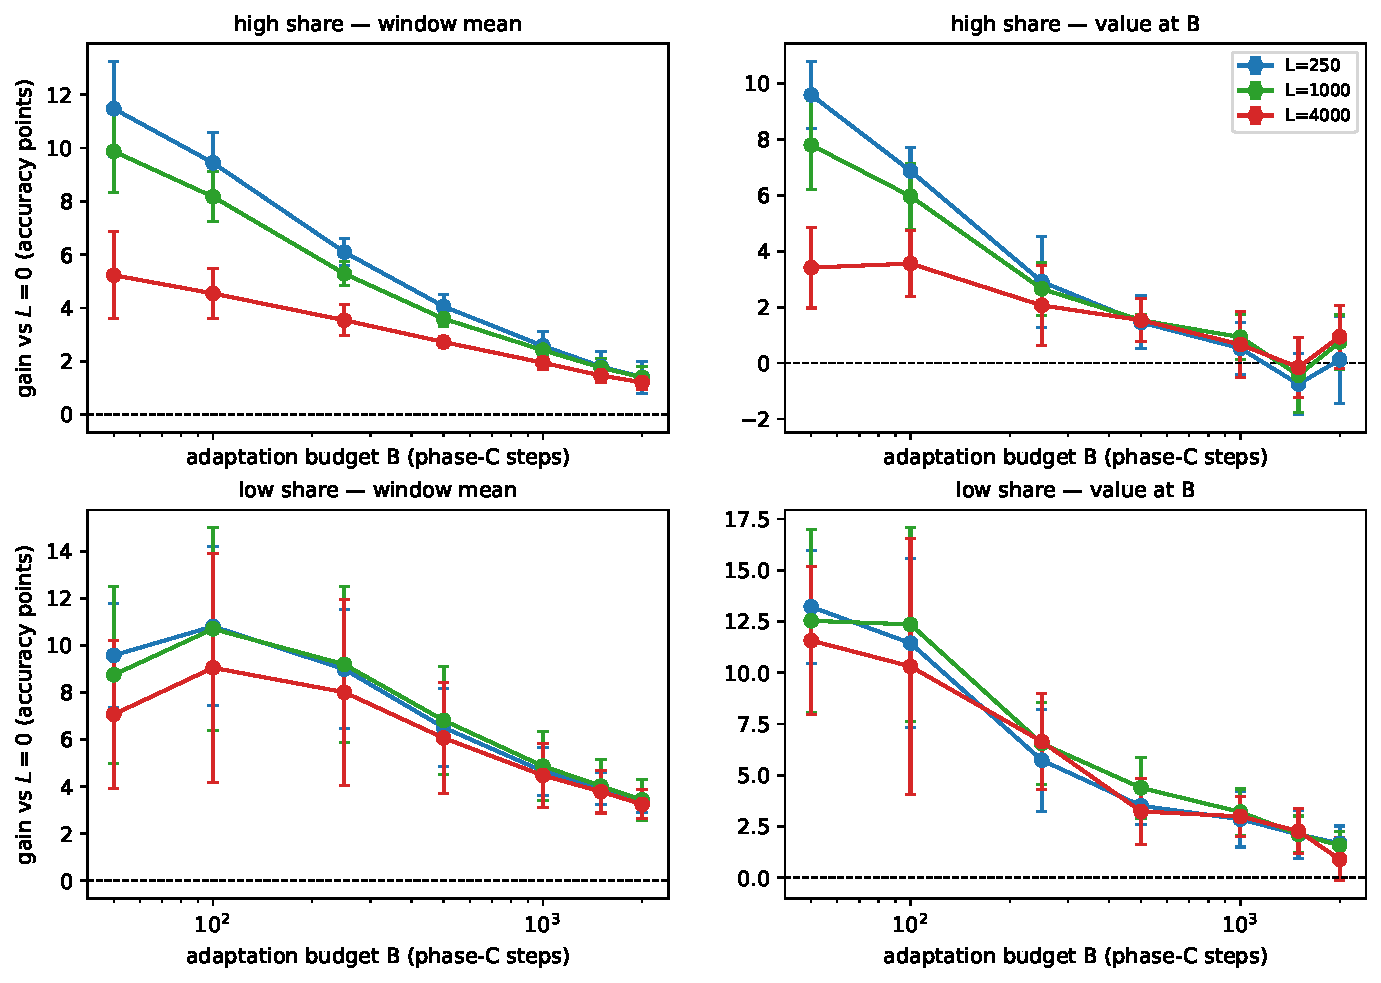
\includegraphics[width=0.98\linewidth]{figures/Figure_3.pdf}
  \caption{Paired gain of every $L>0$ condition over $L{=}0$ as a function of
  the adaptation budget $B$ (log scale). Left column: mean performance over
  the first $B$ steps. Right column: value exactly at step $B$. Top: high
  sharing; bottom: low sharing. Error bars are std over 5 seeds; every point
  at $B\le500$ is positive in all five seeds.}
  \label{fig:budget}
\end{figure}

The pre-registered gate A4 (non-trivial consequence) is met on the full
comparison set: the accuracy range across the four $L$ values and the three
controls is $0.060$ and the NLL range is $0.101$, driven mainly by the
frozen-feature control ($\AccHnd$ accuracy, $\NllHnd$ NLL), i.e.\ the
difference cannot be produced by head retraining alone (E2). The equal-budget
clause (E1) was checked on the subset it can address: over the common set
$L\in\{0,250,1000\}$ the between-$L$ spread is $0.0075$ accuracy /
$0.0210$ NLL without budget equalization and $0.0057$ / $0.0320$ once every
run performs the same number of optimizer steps --- the pattern does not
collapse, so the differences are not a budget artefact. We note plainly that
the \emph{between-$L$} terminal differences are themselves below the rerun
noise floor; the budget and head-only clauses justify the gate, not a terminal
effect claim.

\begin{figure}[t]
  \centering
  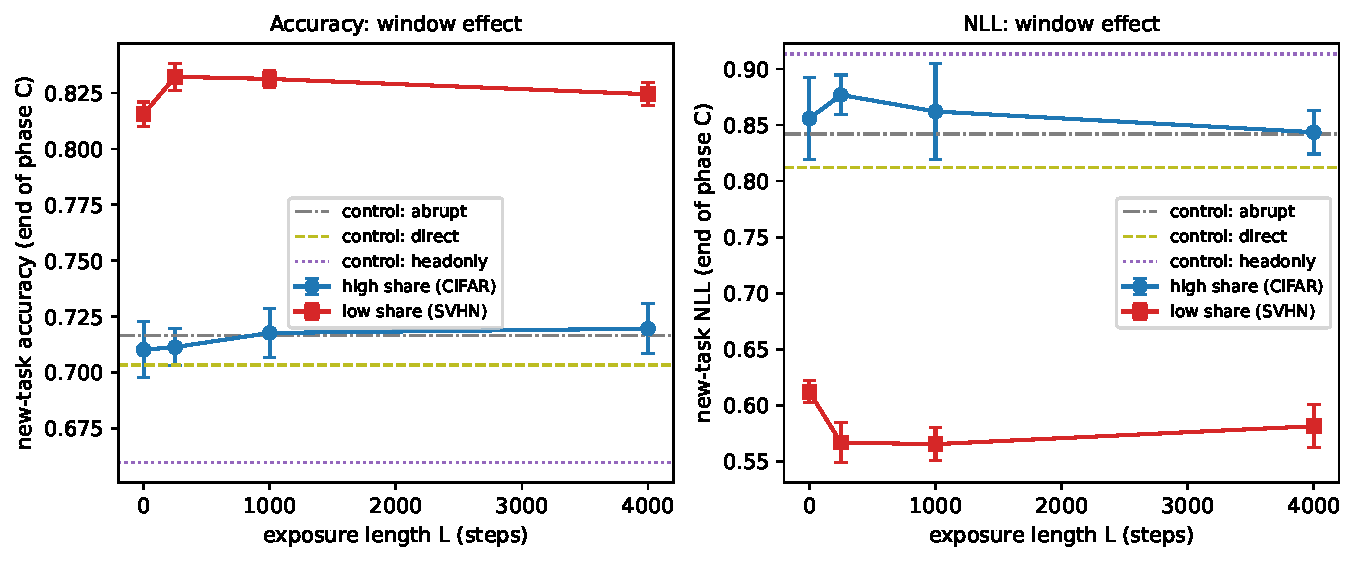
\includegraphics[width=0.98\linewidth]{figures/Figure_4.pdf}
  \caption{Terminal (end of a 2000-step adaptation) new-task performance as a
  function of exposure length $L$, for high and low feature sharing, with the
  controls as horizontal references. Error bars are std over 5 seeds;
  differences are near the measured rerun noise floor (see text).}
  \label{fig:outcome}
\end{figure}

\begin{figure}[t]
  \centering
  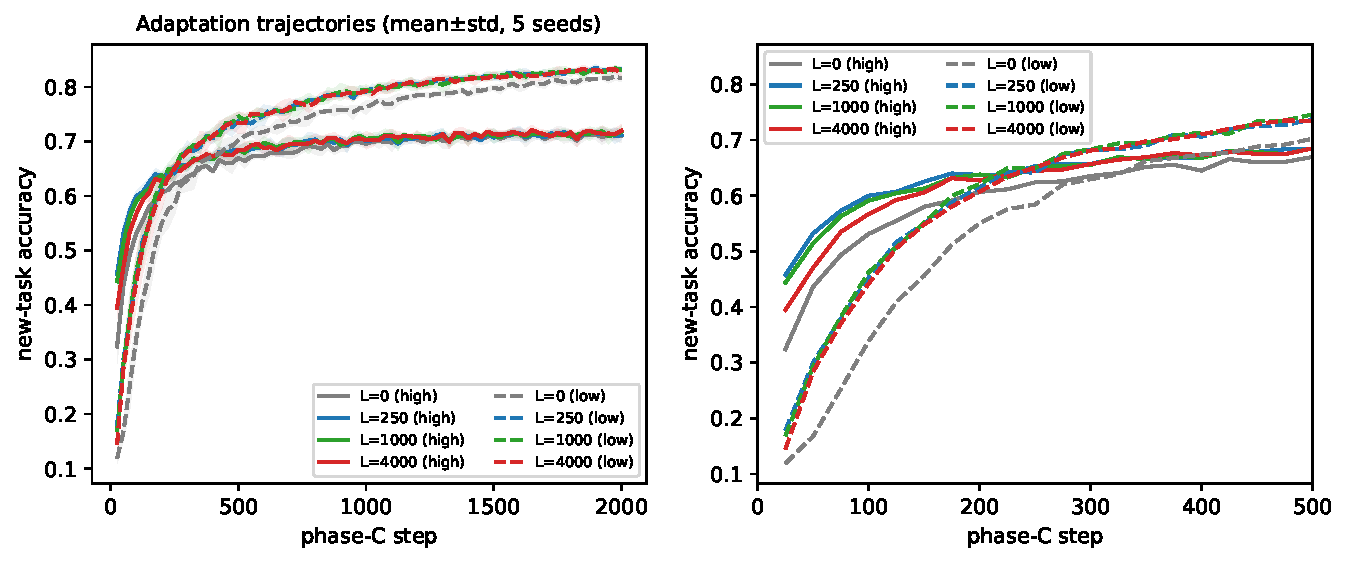
\includegraphics[width=0.98\linewidth]{figures/Figure_5.pdf}
  \caption{Adaptation trajectories. Left: full phase C (mean over 5 seeds,
  shaded band $=$ std). Right: zoom on the first 500 steps, where the
  exposure conditions separate from $L{=}0$ (grey) in both sharing settings.}
  \label{fig:phases}
\end{figure}

\begin{figure}[t]
  \centering
  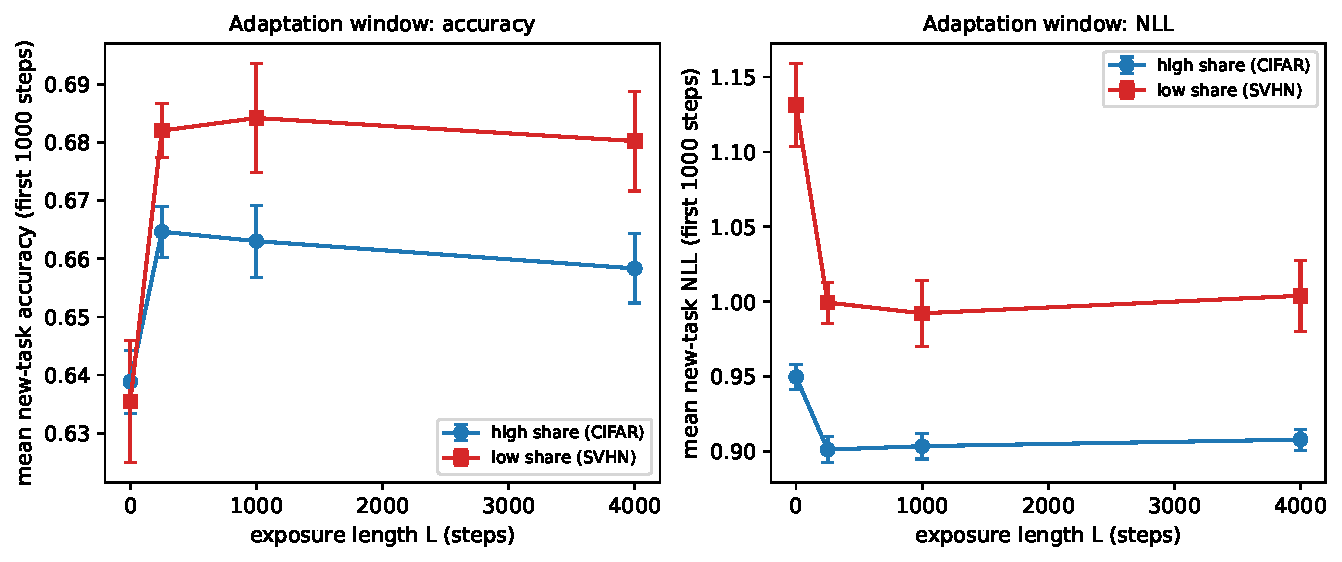
\includegraphics[width=0.98\linewidth]{figures/Figure_6.pdf}
  \caption{Pre-registered adaptation-speed readout: mean new-task accuracy
  (left) and NLL (right) over the first 1000 steps of the adaptation phase as
  a function of exposure length. Error bars are std over 5 seeds.}
  \label{fig:speed}
\end{figure}

\subsection{Controls: the effect is not budget or head retraining}
\label{sec:r-controls}
Table~\ref{tab:controls} reports the controls: the three pre-registered ones
plus the last-layer-reset baseline. Direct training
(no phase A) and the abrupt switch bracket the main sweep; the frozen-feature
control, in which only the head may learn during phase C, lands at
$\AccHnd$, well below the best windowed condition, so the
consequence cannot be attributed to head retraining alone (E2). In the
equal-total-step control (E1), where $L<4000$ conditions are padded with
non-informative $\varepsilon=0$ steps so that every run performs the same
number of optimizer steps, the ordering of the exposure conditions is
preserved.

% ---- tab_controls.tex (auto-generated by analysis/make_tables.py; inlined) ----
% auto-generated by analysis/make_tables.py
\begin{table}[t]
\centering
\caption{Controls: terminal new-task metrics for the three competing-explanation controls (E1 equal budget, E2 head-only retraining) versus the main sweep.}
\label{tab:controls}
\small
\begin{tabular}{llcc}
\toprule
condition & $n$ & new acc & new NLL \\
\midrule
abrupt ($L{=}0$ protocol) & 5 & 0.717 $\pm$ 0.009 & 0.842 $\pm$ 0.023 \\
direct (no phase A) & 5 & 0.703 $\pm$ 0.008 & 0.812 $\pm$ 0.022 \\
headonly (frozen features) & 5 & 0.660 $\pm$ 0.004 & 0.913 $\pm$ 0.009 \\
head reset at switch & 5 & 0.719 $\pm$ 0.013 & 0.849 $\pm$ 0.033 \\
P1 $L{=}0$ & 5 & 0.710 $\pm$ 0.013 & 0.856 $\pm$ 0.037 \\
P1 $L{=}250$ & 5 & 0.711 $\pm$ 0.008 & 0.877 $\pm$ 0.018 \\
P1 $L{=}1000$ & 5 & 0.718 $\pm$ 0.011 & 0.862 $\pm$ 0.043 \\
P1 $L{=}4000$ & 5 & 0.720 $\pm$ 0.011 & 0.844 $\pm$ 0.019 \\
P3 equal-budget $L{=}0$ & 3 & 0.713 $\pm$ 0.003 & 0.843 $\pm$ 0.021 \\
P3 equal-budget $L{=}250$ & 3 & 0.719 $\pm$ 0.005 & 0.874 $\pm$ 0.007 \\
P3 equal-budget $L{=}1000$ & 3 & 0.716 $\pm$ 0.004 & 0.863 $\pm$ 0.010 \\
\bottomrule
\end{tabular}
\end{table}

\paragraph{Comparison with a deliberate head reset.}
The cheapest known intervention --- reinitializing the last layer at the switch
\cite{faia2024reset} --- is the obvious objection: if a released head is what
matters, why expose at all? We ran that arm (P14, five seeds). It is the
fastest adapter we measured: mean new-task accuracy over the first 1000 steps
is $\SpdReset$, against $\SpdHiLzero$ for $L{=}0$ (paired $\DSpdResetLzero$,
\DSpdResetLzeroPos{} seeds) and $\SpdHiLtwoF$ for $L{=}250$ (paired
$\DSpdResetLtwoF$, \DSpdResetLtwoFPos{} seeds); at the endpoint it is
indistinguishable from $L{=}4000$ ($\DAccResetLfourK$ accuracy,
$\DNllResetLfourK$ NLL) and marginally better than $L{=}0$
($\DAccResetLzero$). The comparison cuts both ways. For the mechanism it is
supporting evidence: an \emph{instantaneous} release (reset) and a
\emph{gradual} one (exposure) give the same ordering of outcomes, so the
benefit tracks head release rather than any property of exposure itself. For
practice it is a caveat: exposure recovers most, but not all, of a free reset
--- the residual $\DSpdResetLtwoF$ of adaptation speed is what feature damage
during exposure costs --- and a reset is available only when an intervention
is possible, whereas the window exists precisely for the transitions where
labels are simply unavailable and nothing can be reset.

\subsection{Cross-transplant: what carries the residual consequence?}
\label{sec:r-transplant}
We recombine the head and the feature extractor across exposure lengths at the
end of phase B (same seed, so the two runs share the same protocol through
phase A), then adapt the recombined network to the new task
(Table~\ref{tab:transplant}, Fig.~\ref{fig:transplant}). We analyze the
$2\times2$ design as a factorial with paired seeds:
head main effect (short head minus long head, averaged over features) and
feature main effect (long features minus short features, averaged over heads).

The head main effect is indistinguishable from zero
($+0.0003\pm0.0174$ NLL, $-0.0026\pm0.0090$ accuracy): once the network is
given a full adaptation phase, the state of the head at the moment of the
switch no longer matters --- exactly what the head-only control (E2) predicts
and what rules out a ``the head carries the benefit'' story.
The feature main effect is where the residual difference lives:
$-0.0329\pm0.0144$ NLL, with the same sign in 5/5 seeds, i.e.\ \emph{features
that spent longer under uniform exposure end the adaptation with better NLL},
and $+0.0056\pm0.0077$ accuracy (4/5 seeds). In the first 1000 adaptation
steps the sign flips for accuracy ($-0.0069$, 5/5 seeds), i.e.\ long-exposed
features adapt more slowly at first yet finish ahead.

We emphasize the direction: old-task probe damage is \emph{not} new-task harm
here. Uniform exposure de-specializes the representation away from the old
classes, which is damage measured against the old task (gate A3) but appears
to reduce interference for a new task that reuses the same head slots. The
localization rests on a paired contrast, not on exceeding an absolute noise
floor: within each seed the four cells are recombinations of the same two
checkpoints, so no process-level rerun noise enters the comparison (the
rerun-noise figures quoted in Section~\ref{sec:r-window} quantify \emph{independent
training processes}, a different quantity). The feature main effect is
$-0.0329\pm0.0144$ NLL against a seed-level standard deviation less than half
its magnitude ($|d|\approx2.3$), with the same sign in all five seeds
(one-sided sign test $p=1/32\approx0.031$), whereas the head main effect is
$+0.0003\pm0.0174$ ($d\approx0.02$, a genuine null): the contrast that
localizes the effect, features versus head, is a factor of $\approx100$ in
effect size. We therefore treat the \emph{localization} as supported and the
\emph{magnitude} of the feature effect as a five-seed estimate that
independent replication should confirm.

\paragraph{Replication on the deterministic platform.}
To remove the process-level noise entirely rather than argue about it, we
repeated the whole design on the deterministic platform: the two source runs
($L{=}250$ and $L{=}4000$) were re-executed with deterministic kernels and
saved checkpoints, and the recombinations were re-adapted with a deterministic
phase C, for \DetTN{} seeds. The localization replicates --- feature main
effect $\DetTFeatEff\pm\DetTFeatSd$ NLL with the same sign in \DetTFeatNeg{}
seeds ($|d|=\DetTFeatD$), head main effect
$\DetTHeadEff\pm\DetTHeadSd$ ($|d|=\DetTHeadD$) --- and on this platform
identical configurations are bitwise identical (the property established in
the deterministic replication below), so the process-level rerun noise that
the baseline comparison was measured against is \emph{zero by construction}:
only seed variance remains. The two platforms agree on the effect to within
$0.001$ NLL, i.e.\ the baseline value is not an artefact of noisy sources.

% ---- tab_transplant.tex (auto-generated by analysis/make_tables.py; inlined) ----
% auto-generated by analysis/make_tables.py
\begin{table}[t]
\centering
\caption{Cross-transplant (P4): head and features recombined across exposure lengths, then adapted to the new task.}
\label{tab:transplant}
\small
\begin{tabular}{lccc}
\toprule
combination & $n$ & new acc & new NLL \\
\midrule
native short ($L{=}250$) & 5 & 0.711 $\pm$ 0.008 & 0.877 $\pm$ 0.018 \\
native long ($L{=}4000$) & 5 & 0.720 $\pm$ 0.011 & 0.844 $\pm$ 0.019 \\
short head + long features & 5 & 0.718 $\pm$ 0.005 & 0.852 $\pm$ 0.021 \\
long head + short features & 5 & 0.714 $\pm$ 0.013 & 0.884 $\pm$ 0.030 \\
\bottomrule
\end{tabular}
\end{table}

\begin{figure}[t]
  \centering
  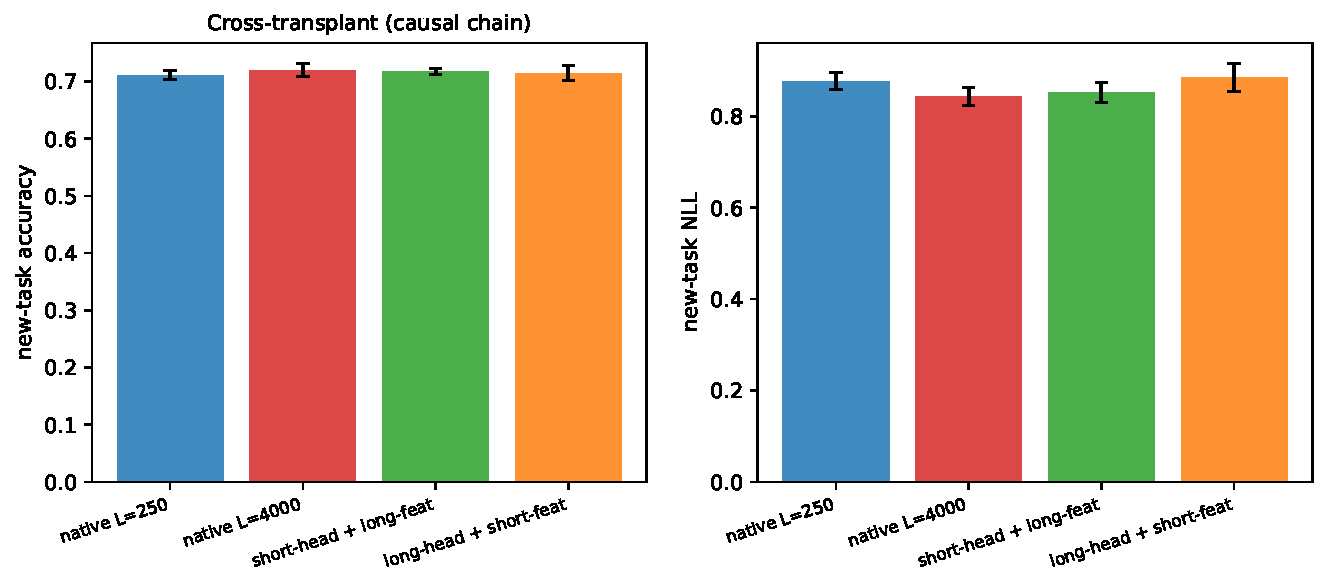
\includegraphics[width=0.98\linewidth]{figures/Figure_7.pdf}
  \caption{Cross-transplant (P4): head and features recombined across exposure
  lengths, then adapted to the new task. Native short/long runs are shown for
  reference.}
  \label{fig:transplant}
\end{figure}

\subsection{Dose--response: the damage tracks target informativeness}
\label{sec:r-e3}
The dose--response arm separates how much class information the exposure
targets still carry (Table~\ref{tab:dose}, Fig.~\ref{fig:e3},
Fig.~\ref{fig:dose}). At a fixed exposure length $L{=}4000$, the
end-of-exposure probe reads $0.853$, $0.735$, $0.714$, $0.675$ and $0.585$ for
$\varepsilon\in\{0,0.9,0.95,0.99,1.0\}$, while the head accuracy reads
$0.885$, $0.817$, $0.783$, $0.707$ and $0.171$ respectively; the
$\varepsilon=0$ arm's feature drift stays below $0.04$ in every seed. Three
things follow.

(i) \emph{Further training alone does nothing}: four thousand extra steps of
plain cross-entropy on the same inputs leave features essentially untouched.
The damage is caused by the loss of label information, not by elapsed
training time (E1 in its strong form).

(ii) \emph{The head only fully releases when the target is
uninformative} --- the A2 condition (head $\le0.50$) is reachable at
$\varepsilon=1.0$ and unreachable at $\varepsilon=0.9$, which is why the
confirmatory blocks use uniform targets; with informative targets the optimum
of the exposure loss still ranks the true class first, so argmax structure
survives by construction.

(iii) \emph{The static label-smoothing account (E3) explains the norms but
not the separation}. The head-weight norm contracts under smoothing in a
dose-dependent way ($7.46$ at $\varepsilon=0$, $6.75$ at $\varepsilon=0.9$,
$6.90$ at $\varepsilon=1.0$), which is exactly what a static neural-collapse
story predicts --- yet at $\varepsilon=0.9$ the norm has contracted and the
head still classifies at $0.817$, and no head/feature window opens. Static
contraction is therefore present but not sufficient; what E3 cannot account
for is the decoupling of head accuracy from feature readability and its
exposure-length dependence. The E4 permutation control returns probe accuracy
at the shuffled-label floor ($\approx0.2$ on the 5-class probe) in the
diagnostic runs, so the probe is not manufacturing readability.

% ---- tab_dose.tex (auto-generated by analysis/make_tables.py; inlined) ----
% auto-generated by analysis/make_tables.py
\begin{table}[t]
\centering
\caption{Dose--response: how much class information the exposure target still carries ($\varepsilon=0$: continued CE; $\varepsilon=1.0$: uniform) controls both head release and feature damage.}
\label{tab:dose}
\small
\begin{tabular}{llrccccc}
\toprule
$\varepsilon$ & $L$ & $n$ & head@endB & probe@endB & $\|W_2\|_{\mathrm{endB}}$ & new acc \\
\midrule
1 & 250 & 5 & 0.437 $\pm$ 0.024 & 0.711 $\pm$ 0.023 & 7.047 $\pm$ 0.245 & 0.711 $\pm$ 0.008 \\
1 & 4000 & 5 & 0.171 $\pm$ 0.018 & 0.585 $\pm$ 0.050 & 6.806 $\pm$ 0.198 & 0.720 $\pm$ 0.011 \\
0.99 & 250 & 3 & 0.481 $\pm$ 0.004 & 0.715 $\pm$ 0.004 & 7.060 $\pm$ 0.041 & 0.719 $\pm$ 0.005 \\
0.99 & 4000 & 3 & 0.707 $\pm$ 0.047 & 0.675 $\pm$ 0.042 & 6.788 $\pm$ 0.037 & 0.720 $\pm$ 0.002 \\
0.95 & 250 & 3 & 0.510 $\pm$ 0.011 & 0.708 $\pm$ 0.016 & 7.096 $\pm$ 0.049 & 0.720 $\pm$ 0.010 \\
0.95 & 4000 & 3 & 0.783 $\pm$ 0.005 & 0.714 $\pm$ 0.012 & 6.851 $\pm$ 0.036 & 0.725 $\pm$ 0.003 \\
0.9 & 250 & 3 & 0.548 $\pm$ 0.028 & 0.728 $\pm$ 0.010 & 7.070 $\pm$ 0.035 & 0.722 $\pm$ 0.003 \\
0.9 & 4000 & 3 & 0.817 $\pm$ 0.004 & 0.735 $\pm$ 0.008 & 6.772 $\pm$ 0.017 & 0.727 $\pm$ 0.007 \\
0 & 4000 & 4 & 0.885 $\pm$ 0.002 & 0.853 $\pm$ 0.004 & 7.562 $\pm$ 0.092 & 0.711 $\pm$ 0.015 \\
\bottomrule
\end{tabular}
\end{table}

\begin{figure}[t]
  \centering
  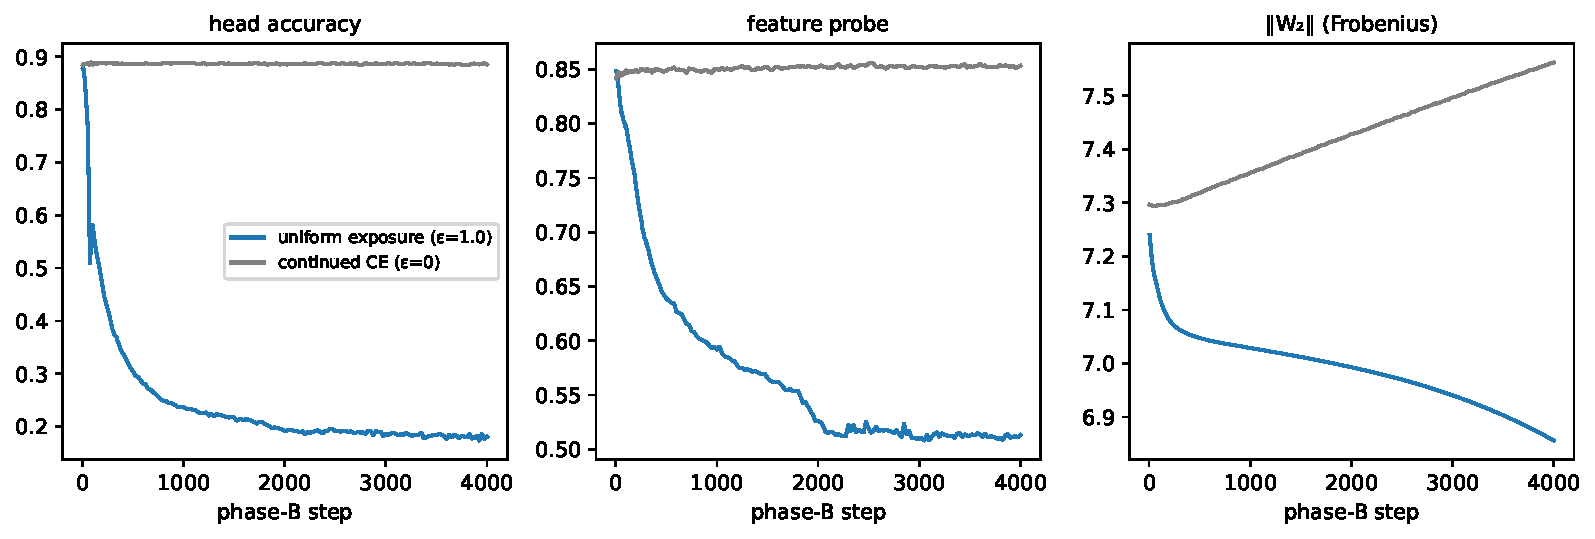
\includegraphics[width=0.98\linewidth]{figures/Figure_8.pdf}
  \caption{Diagnostic runs: head accuracy, feature probe, and head weight
  norm under uniform exposure versus continued cross-entropy ($\varepsilon=0$)
  on the same inputs.}
  \label{fig:e3}
\end{figure}

\subsection{Real sensor drift: the head component transfers, the feature
component does not}
\label{sec:r-sensor}
On the UCI Gas Sensor Array Drift benchmark~\cite{gasdrift} (batch $1\to5$,
128-dimensional responses, small MLP, Table~\ref{tab:sensor},
Fig.~\ref{fig:sensor}) the head
releases exactly as in the image experiments (head accuracy at end of
exposure $0.227$ for $L{=}500$ and $0.158$ for $L{=}2000$), but the
feature probe barely moves ($0.925$ and $0.920$ after exposure, versus
$\approx0.93$ at end of phase A) and terminal accuracy after the drift is
slightly \emph{higher} with exposure ($0.967$ without, $0.974$ with).
The MLP's two hidden layers evidently retain enough structure that 2000
exposure steps do not damage them, so this benchmark corroborates the
head-release component and provides a clear boundary condition for the
feature-damage component: depth/redundancy of the feature map sets the second
timescale. NLL on this benchmark has very large across-seed variance
($0.25$--$0.47$) because several of the four splits are near-saturated, and we
do not interpret it.

% ---- tab_sensor.tex (auto-generated by analysis/make_tables.py; inlined) ----
% auto-generated by analysis/make_tables.py
\begin{table}[t]
\centering
\caption{Real sensor drift (UCI Gas Sensor Array Drift, batch $1\to5$): MLP head/feature state and post-drift performance.}
\label{tab:sensor}
\small
\begin{tabular}{rrcccc}
\toprule
$L$ & $n$ & head@endB & probe@endB & new acc & new NLL \\
\midrule
0 & 4 & -- & -- & 0.967 $\pm$ 0.011 & 0.306 $\pm$ 0.254 \\
500 & 4 & 0.227 $\pm$ 0.059 & 0.925 $\pm$ 0.026 & 0.974 $\pm$ 0.019 & 0.536 $\pm$ 0.472 \\
2000 & 4 & 0.158 $\pm$ 0.015 & 0.920 $\pm$ 0.034 & 0.974 $\pm$ 0.019 & 0.542 $\pm$ 0.444 \\
\bottomrule
\end{tabular}
\end{table}

\begin{figure}[t]
  \centering
  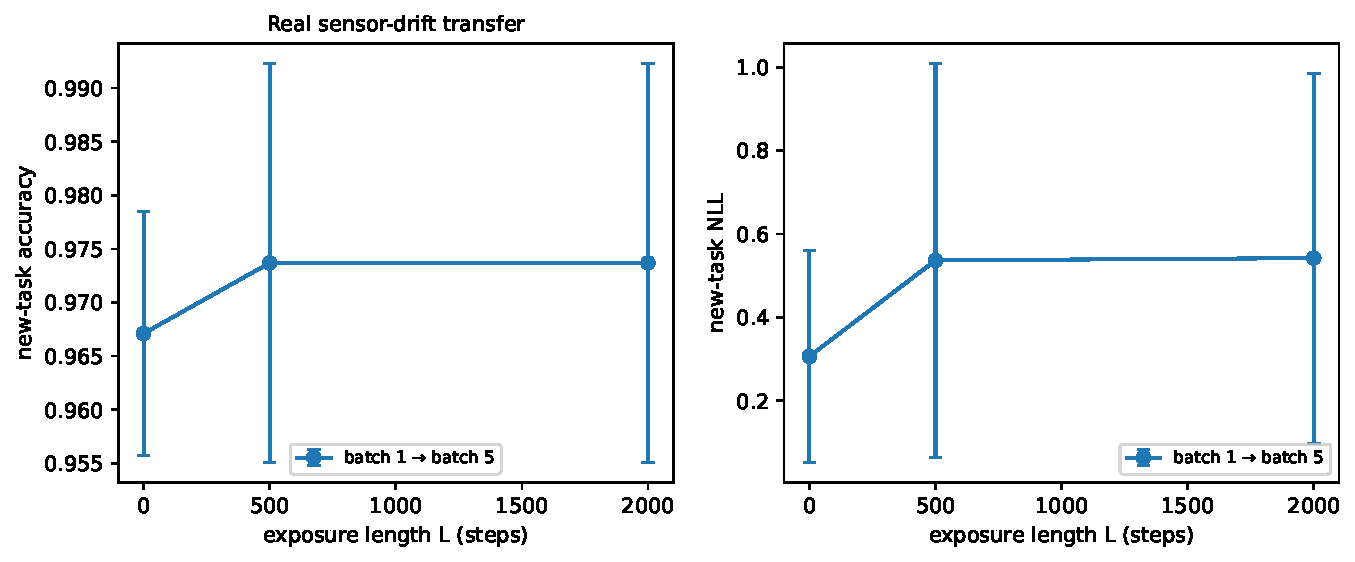
\includegraphics[width=0.98\linewidth]{figures/Figure_9.pdf}
  \caption{Post-drift performance on the UCI Gas Sensor Array Drift benchmark
  as a function of exposure length.}
  \label{fig:sensor}
\end{figure}

\subsection{Scale, dose continuum, and a deterministic replication}
\label{sec:extensions}

\paragraph{Does it hold on a larger model?}
Table~\ref{tab:resnet} repeats the main comparison with ResNet-18 (11.2M
parameters, the architecture named in the pre-registered plan as the scale
extension). The separation survives: \A2ResCount{} of the six
$L\ge250$/seed runs satisfy the A2 condition, with the head at
\HeadResLtwoF\ and the probe at \ProbeResLtwoF\ at the end of a 250-step
exposure, and the adaptation-window ordering is reproduced
($\SpdResLzero$ at $L{=}0$ versus $\SpdResLtwoF$ at $L{=}250$). Terminal NLL
on ResNet-18 is markedly worse than on the small CNN ($\NllResLzero$ versus
$\NllHiLzero$), a reminder that absolute numbers are architecture-specific
even when the mechanism is not. One boundary condition is worth stating
plainly: the probe drop between $L{=}250$ and $L{=}4000$ is only $0.049$
(median $0.058$) on ResNet-18 versus $0.124$ on the CNN, and the adaptation
curve is monotone rather than interior-optimal. Since the window is the
difference between a head-release benefit and a feature-damage cost, a sturdier
feature map shrinks the cost term until the benefit saturates instead of
reversing --- the mechanism predicts exactly this, and the data show it.

\paragraph{Does the damage term track the feature-map width?}
If the window is the difference between a head-release benefit and a
feature-damage cost, both terms should move with the width of the feature map.
We therefore re-ran the exposure comparison at two widths of the same
SmallCNN: $\times0.5$ (33.8k parameters) and $\times2$ (412k), against the
baseline $\times1$ (114k), three seeds each (P16). The cost term moves
monotonically: the probe drop between $L{=}250$ and $L{=}4000$ is
$\ProbeDropWHalf$ at $\times0.5$, $\DropA3$ at $\times1$ and
$\ProbeDropWTwo$ at $\times2$ --- a factor of nine across the range. The
benefit term shifts in time instead of vanishing: at $L{=}250$ the head has
already released in \A2WTwo{} of the $\times2$ runs and in all baseline runs,
but in none of the $\times0.5$ runs (\A2WHalf), because at that width the head
crosses the $0.5$ threshold only between steps \WHalfCrossMin{} and
\WHalfCrossMax{} --- and in one of the three seeds the probe has already fallen
below $0.70$ by then. The window is therefore widest for a wide, redundant
feature map and both late-opening and early-closing for a thin one: this is
exactly the two-term prediction, and it places the architecture boundary
conditions above on a single axis --- ResNet-18's residual path (probe drop
$0.049$) and the two-layer MLP (no measurable drop) are the $\times2$ end of
the same scale.

% ---- tab_resnet.tex (auto-generated by analysis/make_tables.py; inlined) ----
% auto-generated by analysis/make_tables.py
\begin{table}[t]
\centering
\caption{ResNet-18 (11.2M parameters) extension: the head/feature separation and the adaptation window on a larger model.}
\label{tab:resnet}
\small
\begin{tabular}{lrcccccc}
\toprule
$L$ & $n$ & new acc & new NLL & speed$_{1000}$ & head@endB & probe@endB & A2 \\
\midrule
0 & 3 & 0.701 $\pm$ 0.007 & 1.154 $\pm$ 0.019 & 0.649 $\pm$ 0.004 & -- & -- & 0 \\
250 & 3 & 0.708 $\pm$ 0.013 & 1.126 $\pm$ 0.033 & 0.662 $\pm$ 0.002 & 0.211 $\pm$ 0.007 & 0.676 $\pm$ 0.017 & 3 \\
4000 & 3 & 0.713 $\pm$ 0.007 & 1.121 $\pm$ 0.036 & 0.668 $\pm$ 0.005 & 0.138 $\pm$ 0.022 & 0.627 $\pm$ 0.013 & 3 \\
\bottomrule
\end{tabular}
\end{table}

\paragraph{How much information must the target lose?}
Figure~\ref{fig:dose} and Table~\ref{tab:dose} extend the dose--response from
two anchor points to a continuum of target information content. Head release
is threshold-like: after a 4000-step exposure the head still classifies at
$0.885$ ($\varepsilon=0$), $0.817$ ($0.9$), $0.783$ ($0.95$) and $0.707$
($0.99$), yet collapses to $0.171$ exactly at $\varepsilon=1.0$ --- because
for any $\varepsilon<1$ the optimum of the exposure loss still ranks the true
class first. Feature damage, in contrast, grows smoothly as
$\varepsilon\to1$ ($0.853\to0.735\to0.714\to0.675\to0.585$ probe), and the
A2 window opens dose-dependently ($0/3\to1/3\to3/3\to5/5$ seed hits at
$L{=}250$). The head-weight norm contracts monotonically between
$\varepsilon=0$ and $0.9$ and then flattens, which is consistent with a static
label-smoothing account of the norm but not of the accuracy decoupling.

\begin{figure}[t]
  \centering
  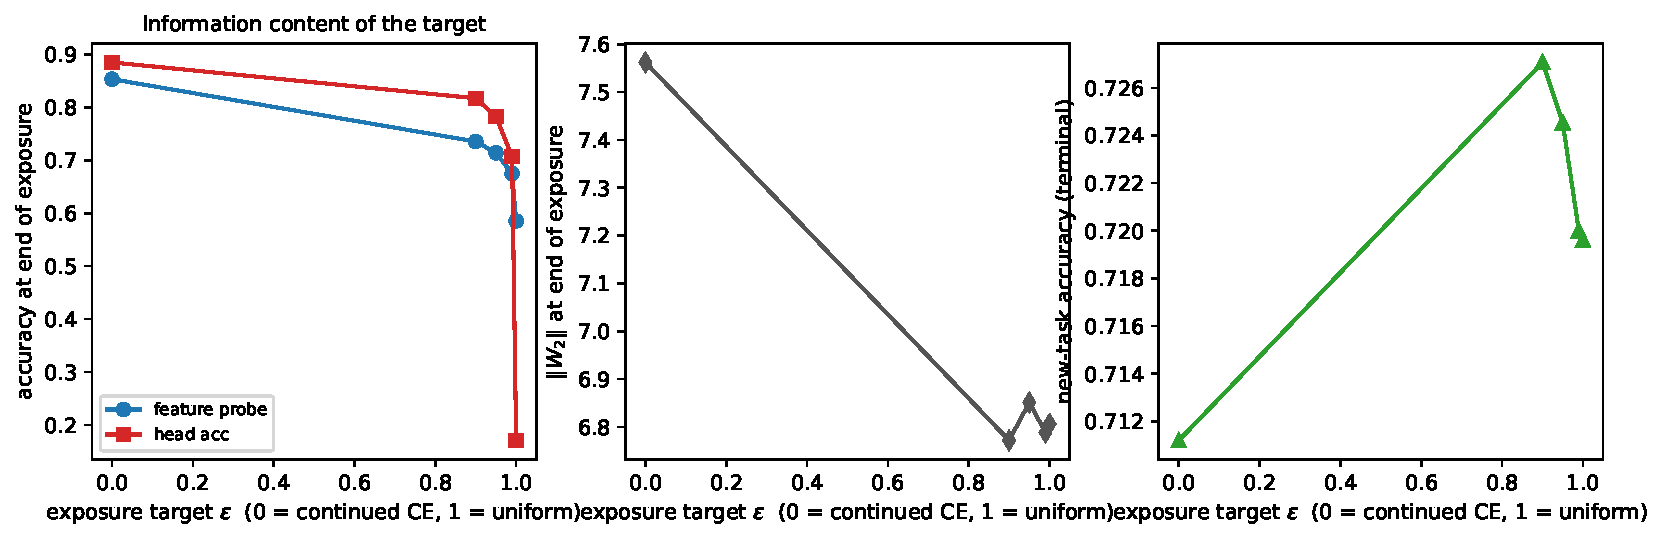
\includegraphics[width=0.98\linewidth]{figures/Figure_10.pdf}
  \caption{Dose--response at fixed exposure length $L{=}4000$: probe and head
  accuracy (left), head-weight norm (center), and terminal new-task accuracy
  (right) as a function of the information content of the exposure target.}
  \label{fig:dose}
\end{figure}

\paragraph{Deterministic replication.}
We re-ran the main conditions with deterministic kernels (cuDNN deterministic
mode, TF32 off, and a forward-identical replacement of the adaptive average
pool by a fixed $2\times2$ average pool, which removes the only atomic-add
backward in the graph). \DetPairs{} pairs of runs with byte-identical
configurations now produce metric streams that are \emph{bitwise identical}
(max $|\Delta|=\DetMaxDelta$ over all rows; every pair listed in
Table~\ref{tab:det}), so the process-level rerun noise
measured in Section~\ref{sec:r-window} is eliminated by construction. Pooling
all \DetSeeds{} deterministic seeds (5 original + 5 added), the terminal
readout is $L{=}0$/$250$/$4000$ at
$\AccDet10Lzero$/$\AccDet10LtwoF$/$\AccDet10LfourK$ accuracy with an
endpoint range of only $\DetLRrange$ points, while the adaptation-window gain
of $L{=}250$ over $L{=}0$ is $+\DetWindowGain$ points and positive in
\DetWindowPos\ seeds. On this benchmark family the endpoint effect is thus
statistically indistinguishable from zero once procedural noise is removed;
the effect that survives is the adaptation-speed effect.

% ---- tab_det.tex (auto-generated by analysis/make_tables.py; inlined) ----
% auto-generated by analysis/make_tables.py
\begin{table}[t]
\centering
\caption{Deterministic-kernel replication (P10): two independent runs with identical configuration produce bitwise-identical metric streams (max $|\Delta|$ over all rows), so terminal differences are no longer contaminated by process-level rerun noise.}
\label{tab:det}
\small
\begin{tabular}{rrrc}
\toprule
seed & $L$ & rows & max $|\Delta|$ \\
\midrule
42 & 0 & 280 & 0.0e+00 \\
42 & 250 & 330 & 0.0e+00 \\
42 & 4000 & 504 & 0.0e+00 \\
123 & 0 & 280 & 0.0e+00 \\
123 & 250 & 330 & 0.0e+00 \\
123 & 4000 & 504 & 0.0e+00 \\
\bottomrule
\end{tabular}
\end{table}

\subsection{External validity: a larger label space and a second cross-domain
partner}
\label{sec:external}
Across all extensions the invariant is the \emph{ordering} --- the head
releases first --- and it holds in every single run; what varies is the size
of the feature-damage term, which the two-term (benefit $-$ damage) picture
predicts from the redundancy of the feature map. The paragraphs below separate
these two aspects: the invariants, and then the moderator.

\paragraph{CIFAR-100 (25 old / 25 new fine classes).}
Table~\ref{tab:c100} and Fig.~\ref{fig:external} repeat the protocol with ten
times the label space and the official train/test split, for both
architectures. The separation
replicates in \emph{every single run}: \A2CnnC100\ (SmallCNN) and \A2RnC100\
(ResNet-18) of the six $L\ge250$ runs per model satisfy the A2 condition.
What differs is the cost term. For SmallCNN the probe at the end of exposure
falls from \ProbeCnnC100LtwoF\ ($L{=}250$) to \ProbeCnnC100LfourK\
($L{=}4000$) --- a paired drop of $0.147$ --- and the new task (25 classes,
feature-hungry) pays for it: terminal accuracy decreases with exposure
($\AccCnnC100Lzero\to\AccCnnC100LtwoF\to\AccCnnC100LfourK$) and NLL increases
($\NllCnnC100Lzero\to\NllCnnC100LfourK$), while the adaptation window is still
visible in the first 1000 steps ($\SpdCnnC100Lzero\to\SpdCnnC100LtwoF$).
ResNet-18's features barely move (probe drop $0.015$), and correspondingly
its outcome is flat across $L$. The sign of the endpoint effect therefore
tracks \emph{how much the new task needs the features}, exactly as the
two-term (benefit $-$ damage) picture predicts.

% ---- tab_c100.tex (auto-generated by analysis/make_tables.py; inlined) ----
% auto-generated by analysis/make_tables.py
\begin{table}[t]
\centering
\caption{External validity on CIFAR-100 (25 old / 25 new fine classes, official split, head slots reused): the head/feature separation and the adaptation window replicate on a harder, larger-labelspace benchmark.}
\label{tab:c100}
\small
\begin{tabular}{llrccccccc}
\toprule
model & $L$ & $n$ & endA & new acc & new NLL & speed$_{1000}$ & head@endB & probe@endB & A2 \\
\midrule
smallcnn & 0 & 3 & 0.932 $\pm$ 0.010 & 0.827 $\pm$ 0.003 & 0.559 $\pm$ 0.008 & 0.768 $\pm$ 0.001 & -- & -- & 0 \\
smallcnn & 250 & 3 & 0.921 $\pm$ 0.003 & 0.816 $\pm$ 0.010 & 0.605 $\pm$ 0.039 & 0.784 $\pm$ 0.004 & 0.431 $\pm$ 0.024 & 0.867 $\pm$ 0.008 & 3 \\
smallcnn & 4000 & 3 & 0.923 $\pm$ 0.002 & 0.805 $\pm$ 0.015 & 0.705 $\pm$ 0.027 & 0.765 $\pm$ 0.006 & 0.147 $\pm$ 0.030 & 0.720 $\pm$ 0.074 & 3 \\
resnet18 & 0 & 3 & 0.919 $\pm$ 0.012 & 0.818 $\pm$ 0.016 & 0.721 $\pm$ 0.043 & 0.765 $\pm$ 0.002 & -- & -- & 0 \\
resnet18 & 250 & 3 & 0.904 $\pm$ 0.004 & 0.809 $\pm$ 0.008 & 0.753 $\pm$ 0.016 & 0.769 $\pm$ 0.002 & 0.217 $\pm$ 0.012 & 0.760 $\pm$ 0.033 & 3 \\
resnet18 & 4000 & 3 & 0.913 $\pm$ 0.011 & 0.812 $\pm$ 0.019 & 0.739 $\pm$ 0.109 & 0.779 $\pm$ 0.004 & 0.191 $\pm$ 0.015 & 0.745 $\pm$ 0.031 & 3 \\
\bottomrule
\end{tabular}
\end{table}

\paragraph{Second cross-domain partner: Fashion-MNIST.}
Replacing SVHN by Fashion-MNIST in the low-sharing arm
(Table~\ref{tab:fmnist}) reproduces every qualitative fact: \A2Fmn\ of six runs
satisfy A2, the probe decays with exposure
(\ProbeFmnLtwoF$\to$\ProbeFmnLfourK), the adaptation window opens
($\SpdFmnLzero\to\SpdFmnLtwoF$), and at the endpoint the longest exposure is
slightly \emph{best} in NLL ($\NllFmnLfourK$ versus $\NllFmnLzero$).

% ---- tab_fmnist.tex (auto-generated by analysis/make_tables.py; inlined) ----
% auto-generated by analysis/make_tables.py
\begin{table}[t]
\centering
\caption{Second cross-domain partner for the low-sharing arm: CIFAR-10 (old) $\to$ Fashion-MNIST (new).}
\label{tab:fmnist}
\small
\begin{tabular}{lrcccccc}
\toprule
$L$ & $n$ & new acc & new NLL & speed$_{1000}$ & head@endB & probe@endB & A2 \\
\midrule
0 & 3 & 0.884 $\pm$ 0.006 & 0.331 $\pm$ 0.016 & 0.837 $\pm$ 0.003 & -- & -- & 0 \\
250 & 3 & 0.884 $\pm$ 0.003 & 0.333 $\pm$ 0.009 & 0.849 $\pm$ 0.001 & 0.459 $\pm$ 0.004 & 0.717 $\pm$ 0.007 & 3 \\
4000 & 3 & 0.890 $\pm$ 0.005 & 0.309 $\pm$ 0.009 & 0.846 $\pm$ 0.001 & 0.167 $\pm$ 0.009 & 0.595 $\pm$ 0.024 & 3 \\
\bottomrule
\end{tabular}
\end{table}

\paragraph{Ten seeds on the deterministic platform.}
Finally we pool the deterministic runs over ten seeds: the adaptation-window
gain of $L{=}250$ over $L{=}0$ is $+\DetWindowGain$ accuracy points on average
and positive in \DetWindowPos\ seeds, while the \emph{endpoint} range across
$L\in\{0,250,4000\}$ is only $\DetLRrange$ points
($\AccDet10Lzero$/$\AccDet10LtwoF$/$\AccDet10LfourK$). On this benchmark family
the honest summary is therefore: \emph{exposure reliably buys adaptation
speed and never meaningfully changes the endpoint --- unless the new task is
large enough to be feature-limited (CIFAR-100), in which case long exposure
costs accuracy at the endpoint while still helping early.}

\begin{figure}[t]
  \centering
  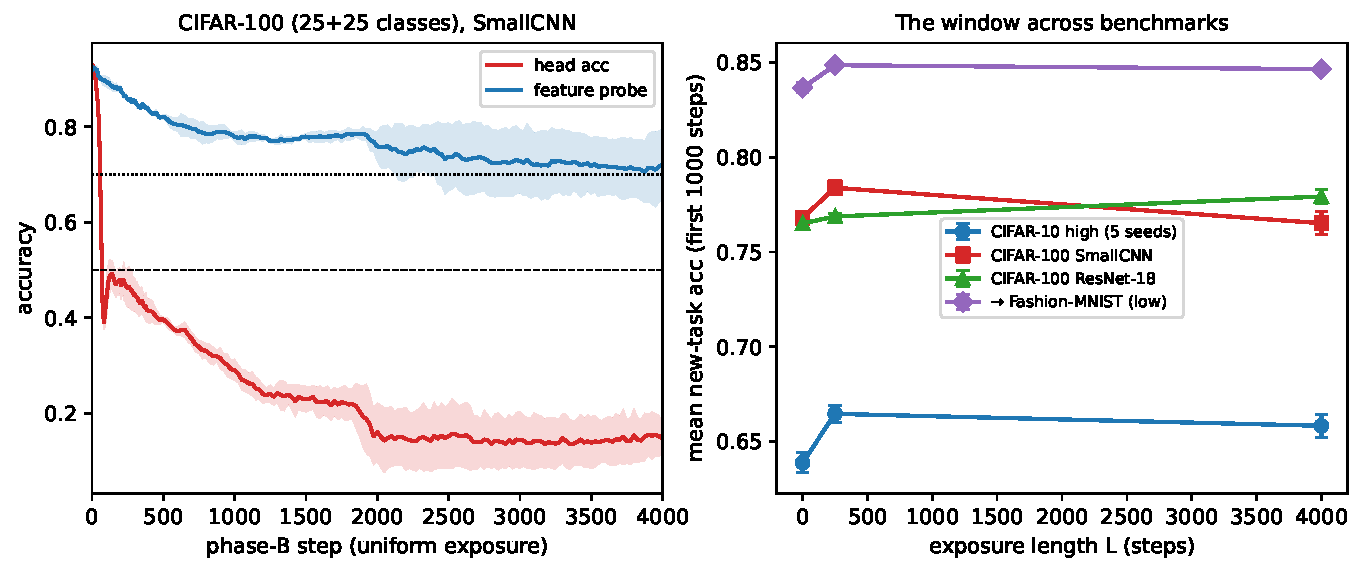
\includegraphics[width=0.98\linewidth]{figures/Figure_11.pdf}
  \caption{External validity. Left: head and feature trajectories under uniform
  exposure on CIFAR-100 (SmallCNN, $L{=}4000$, mean over 3 seeds). Right: the
  adaptation-window readout across benchmarks, including both CIFAR-100
  architectures and the Fashion-MNIST arm.}
  \label{fig:external}
\end{figure}

\subsection{Resources}
\label{sec:r-resources}
All runs were executed on a single RTX 5060 Laptop GPU (8.5\,GB).
Table~\ref{tab:resources} reports measured resources: \NumConfirmatory{}
confirmatory runs in total (\NumExecuted{} runs executed overall: one timing
run, \NumCalibration{} calibration/smoke runs and \NumExtended{}
post-hoc robustness runs outside the pre-registered gate set), mean wall time
\WallMean\,s per run
(max \WallMax\,s), peak RSS \PeakRss\,MB, peak GPU memory \PeakGpu\,MB. The
whole campaign fits in a few GPU-hours, which made it possible to run the
pre-registered gates without degradation.

% ---- tab_resources.tex (auto-generated by analysis/make_tables.py; inlined) ----
% auto-generated by analysis/make_tables.py
\begin{table}[t]
\centering
\caption{Measured resources over all formal runs (RTX 5060 Laptop, 8.5\,GB).}
\label{tab:resources}
\small
\begin{tabular}{lcc}
\toprule
metric & value & unit \\
\midrule
runs measured & 190 & -- \\
wall per run (mean) & 204.6 & s \\
wall per run (max) & 803.5 & s \\
peak RSS (max) & 2320 & MB \\
peak GPU mem (max) & 782 & MB \\
\bottomrule
\end{tabular}
\end{table}

% ===========================================================================
\section{Discussion}
\label{sec:discussion}

\paragraph{Why a window exists --- a threshold-crossing argument.}
Write the head rows as $w_i = \bar w + \delta_i$ with $\sum_i \delta_i=0$, and
let $p=\mathrm{softmax}(W_2\phi)$, $t=$ uniform under exposure. Two gradients
govern the transient:
\begin{equation}
\frac{\partial \mathcal L}{\partial W_2} = (p-t)\,\phi^{\top},
\qquad
\frac{\partial \mathcal L}{\partial \phi} = W_2^{\top}(p-t)
= \textstyle\sum_i \delta_i\,(p_i-t_i),
\end{equation}
where the $\bar w$ term cancels exactly because $\sum_i(p_i-t_i)=0$. Three
consequences follow, each with a measured counterpart.

\emph{(i) The features are self-gated by the head's anisotropy.} Feature
learning is driven only by $\delta_i$, i.e.\ only by how \emph{unequal} the head
rows still are; as the head equalizes, feature drift shuts off even though the
loss is still non-zero. This predicts the concave probe curve of
Fig.~\ref{fig:traj}: most damage accumulates while the head is still
anisotropic (first few hundred steps), then saturates --- exactly what is
observed, and why the probe drop from $L{=}250$ to $L{=}4000$ is only
$\DropA3$ while the drop from $L{=}0$ to $L{=}250$ is far larger.

\emph{(ii) The window is a gap between two thresholds, not two ODEs.} Head
readability fails when row dispersion falls below the classification margin
$m$ --- a \emph{thin} threshold in the head coordinate; the readout is a linear
classifier, and for such models the margin structure, rather than any global
loss value, governs the dynamics of gradient-based training
\cite{soudry2018implicit}. Probe readability, in contrast, fails only after the
accumulated $\int\|\delta\|\,dt$ has moved $\phi$ beyond its robustness radius
$R$ --- a \emph{large} threshold in the feature coordinate. The head crosses
first because its margin is small and it receives $O(\|\phi\|)$ gradients
directly.

\emph{(iii) All crossing times scale as $1/\eta$.} Under a fixed exposure
schedule the trajectory depends on the step size only through $\eta t$, so
both thresholds are crossed at times $\propto1/\eta$: the window must widen as
the exposure learning rate shrinks and vanish as it grows. The pre-run
calibration (S-exposure2, $\eta\in\{10^{-3},3{\times}10^{-4},10^{-4}\}$) gives
head crossings at steps $10/25/75$ and probe crossings at $20/70/325$, i.e.\
window durations $10\to45\to250$ --- widening by $25\times$ for a $10\times$
reduction in $\eta$ (at least the predicted $1/\eta$, with the excess because
larger steps also push the head past its margin before the probe can register
damage). At $\eta=10^{-3}$ the window collapses to two evaluation points and
the A3 drop vanishes ($0.009$), as the model predicts.

\paragraph{The same argument in words.}
The exposure objective with a uniform target has a degenerate optimum: any
parameter setting that maps all inputs to the same logits is optimal. The head
is a single linear map and reaches that manifold quickly, whereas the feature
extractor is a deep, redundant map whose class information is only
\emph{incidentally} harmful to the exposure loss; it therefore decays slowly.
Because the head's contribution to the loss is directly visible in the logits
while feature damage requires the accumulated movement of many parameters, the
two timescales separate by more than an order of magnitude in our
measurements. The consequence for downstream learning is a genuine trade-off:
releasing the head removes an obstacle for the new task, while continued
exposure keeps changing the representation the new task would like to build
on.

\paragraph{Damage to the old task is not harm to the new task.}
A nuance the cross-transplant forces on us: the feature state that scores
worst on the \emph{old}-task probe (long exposure) finishes ahead on the
\emph{new}-task NLL, while scoring slightly worse in the first thousand
adaptation steps. Uniform exposure trades old-task readability for
de-specialization, and de-specialization can be exactly what a new task that
reuses the same output slots wants. Any practical stopping rule therefore has
to name its objective: probe the old task (stop early), or adapt fast to the
new task (stop as soon as the head has released), rather than maximize
either signal alone.

\paragraph{A stopping rule for label-scarce transitions.}
Combining the two effects yields an operational rule that costs almost
nothing to monitor: expose until the \emph{head} stops reading the old task
while the \emph{probe} still does, then switch. In our protocol that is
roughly $L\approx250$--$1000$ steps, the interval in which both criteria hold
simultaneously. The current task's own accuracy is useless as a stopping
signal --- it sits near chance for the entire window --- and continuing past
the window buys nothing at the endpoint ($\DetLRrange$ accuracy points across
$L$ on the deterministic platform) while risking the feature cost observed on
feature-limited new tasks. Because all crossing times scale as $1/\eta$, the
rule transfers across learning rates after a short calibration that measures
the two crossing times once: switch anywhere between them.

\paragraph{Limitations.}
First, the claim ceiling frozen before execution permits only ``evidence of a
separable mechanism on these benchmarks'': the study is pre-registered with
\NumConfirmatory{} confirmatory runs, but it is single-lab, single-GPU, and
its seeds share one data ordering.
Second, terminal between-condition differences are at or below the measured
rerun noise floor (independent processes with identical protocols differ by up
to $0.024$ accuracy and $0.046$ NLL), so we claim the adaptation-window effect
and not a terminal effect; a larger or deterministic apparatus is required for
the latter. Third, the exposure target is exactly uniform; realistic
transitions (noisy, ambiguous, or coarser labels) sit between
$\varepsilon=0.9$ and $\varepsilon=1.0$ and we have not mapped that continuum.
Fourth, the feature-damage timescale is set by the feature map: it appears for
the CNN on images but not for a two-layer MLP on sensor data, so any transfer
of the stopping rule to a new architecture needs a probe-based pilot first.
Fifth, an independent cross-model code review was completed and did find real
defects (the equal-budget clause of gate A4 was computed but not wired into the
verdict; the head-only exclusion used ``any'' instead of ``every''
condition). Both were fixed and the gates re-evaluated --- the verdict is
unchanged --- but it is a reminder that pre-registration is only as good as its
implementation. Independent replication of the \emph{results}, a theoretical
account of the two timescales, and a lower-noise apparatus for terminal
effects are required before any claim beyond the pre-registered claim ceiling.

% ===========================================================================
\section{Conclusion}
\label{sec:conclusion}
Treating a label-scarce task transition as a measurable object --- rather than
as an inconvenience --- reveals structure that terminal analyses cannot see:
the classifier head and the feature extractor de-specialize on different
timescales, the separation defines a finite window, and the window has a
non-monotone effect on later adaptation that is carried by the features. For
practitioners the message compresses to one sentence: \emph{stop exposing when
the head stops reading the old task and before the probe begins to fall} --- a
rule that current-task accuracy cannot give you, and one whose cost of
checking is a single linear probe. We hope the protocol, the pre-registered
gates, and the released artefacts make this an easy phenomenon to replicate or
refute.

\section*{Reproducibility and pre-registration statement}
The plan, deviations log, queue, and orchestration state are released with the
code. Gate thresholds and the claim ceiling were frozen before the
confirmatory blocks; every deviation (task class split, exposure form, exposure
learning rate, evaluation density) is recorded with its calibration evidence in
\texttt{pilot/DEVIATIONS.md}. Figures are vector PDFs generated by
\texttt{analysis/visualization.py}; all numbers in this manuscript are injected
by \texttt{analysis/paper_macros.py} from the raw \texttt{metrics.jsonl} files.

\section*{Data availability}\begingroup\sloppy
Underlying image and sensor datasets are third-party and are cited as data
references in the reference list. The code, configurations, raw per-evaluation
metrics and analysis scripts supporting this study are released in the GitHub
repository \url{https://github.com/python123flask/C1-head-feature-window} and
archived at Zenodo~\cite{xliu2026c1release} (version v2.1; version DOI
\url{https://doi.org/10.5281/zenodo.23162540}, concept DOI
\url{https://doi.org/10.5281/zenodo.23157274}). All reported numbers are
generated from the raw \texttt{metrics.jsonl} files in that archive by the
released analysis scripts.
\endgroup

\section*{Declaration of competing interest}
The author declares that there are no known competing financial interests or
personal relationships that could have appeared to influence the work reported
in this paper.

\section*{Funding}
This research did not receive any specific grant from funding agencies in the
public, commercial, or not-for-profit sectors.
% 如获资助，改用指南标准格式并删除上面一句：
% Funding: This work was supported by [Funder] [grant numbers xxxx, yyyy].

\section*{CRediT authorship contribution statement}
% 指南要求（"Corresponding authors are required to acknowledge co-author
% contributions using CRediT roles"）。以下按单作者填写；如实际有合著者，
% 请把每人的真实角色分别列出（用分号分隔），只保留实际承担的角色。
\textbf{Xianzhe Liu:} Conceptualization, Methodology, Software, Investigation,
Formal analysis, Data curation, Validation, Resources, Visualization,
Writing --- original draft, Writing --- review \& editing.

\section*{Declaration of generative AI and AI-assisted technologies in the manuscript preparation process}
During the preparation of this work the author used an LLM-based AI assistant
(DeepSeek, accessed through the DeepSeek Harness environment) in order to draft
and revise manuscript text, and to implement, debug and review the experiment,
analysis and plotting code. All quantitative results reported here were
produced by the released code from measurements recorded during the runs; all
figures were rendered from those measurements by the released plotting
scripts; and reference metadata were cross-checked against arXiv, ACL
Anthology and OpenAlex records, with the one identifier that could not be
verified flagged in the reference list. After using this tool, the author
reviewed and edited the content as needed and takes full responsibility for the
content of the published article. No generative AI tool was used to create or
alter any image in this manuscript.

% ===========================================================================
\begin{thebibliography}{99}

% ---------- 本工作直接相关的前作 ----------
\bibitem{guo2025cross}
L.~Guo, G.~Andriopoulos, Z.~Zhao, S.~Ling, Z.~Dong, K.~Ross,
``Cross entropy versus label smoothing: a neural collapse perspective,''
Transactions on Machine Learning Research, 2025. arXiv:2402.03979.

\bibitem{wang2025maxsup}
Y.~Zhou, H.~Li, Z.-Q.~Cheng, X.~Yan, Y.~Dong, M.~Fritz, M.~Keuper,
``MaxSup: overcoming representation collapse in label smoothing,'' in
\emph{Advances in Neural Information Processing Systems 38 (NeurIPS)}, 2025
(oral). DOI: 10.52202/085713-5385.

\bibitem{meister2020generalized}
C.~Meister, E.~Salesky, R.~Cotterell, ``Generalized entropy regularization
or: there's nothing special about label smoothing,'' in \emph{Proc. Annual
Meeting of the Association for Computational Linguistics (ACL)}, 2020,
pp. 6870--6886. DOI: 10.18653/v1/2020.acl-main.615.

\bibitem{szegedy2016rethinking}
C.~Szegedy, V.~Vanhoucke, I.~Sermanet, J.~Sherry, C.~Szegedy,
``Rethinking the Inception architecture for computer vision,'' in \emph{Proc.
IEEE Conf. Computer Vision and Pattern Recognition (CVPR)}, 2016,
pp. 2818--2826.

\bibitem{muller2019label}
K.~M\"{u}ller, I.~Kornblith, G.~Hinton, ``When does label smoothing help?,''
in \emph{Advances in Neural Information Processing Systems 32 (NeurIPS)},
2019.

\bibitem{papyan2020prevalence}
V.~Papyan, X.~Y.~Han, D.~L.~Donoho, ``Prevalence of neural collapse during
the terminal phase of deep learning training,''
Proceedings of the National Academy of Sciences 117(40) (2020) 24652--24663.
DOI: 10.1073/pnas.2015509117.

\bibitem{joudaki2026barriers}
A.~Joudaki, G.~Lanzillotta, M.~S.~Razlighi, I.~Mirzadeh, K.~Alizadeh,
T.~Hofmann, M.~Farajtabar, F.~Faghri,
``Barriers for learning in an evolving world: mathematical understanding of
loss of plasticity,'' in \emph{Proc. International Conference on Learning
Representations (ICLR)}, 2026. arXiv:2510.00304.

\bibitem{kumar2022loss}
S.~Kumar, H.~Yao, D.~Jayaraman, G.~Kornblith, S.~Ma, R.~Grosse, J.~Ba,
``Understanding loss of plasticity in deep neural networks and its cure,''
in \emph{Advances in Neural Information Processing Systems 35 (NeurIPS)},
2022.

\bibitem{faia2024reset}
L.~Frati, N.~Traft, J.~Clune, N.~Cheney,
``Reset it and forget it: relearning last-layer weights improves continual
and transfer learning,'' in \emph{Frontiers in Artificial Intelligence and
Applications (ECAI)}, 2024. DOI: 10.3233/FAIA240840.

\bibitem{ren2026learning}
Y.~Ren, W.~Deng, G.~Hong, C.~Lyle, Y.~Gal,
``Learning dynamics of continual learning: a unified view of data
attribution, forgetting, and plasticity loss,'' arXiv:2609.33620, 2026
(concurrent work).

% ---------- 持续学习与可塑性 ----------
\bibitem{delange2021survey}
M.~De Lange, R.~Aljundi, M.~Masana, S.~Parisot, X.~Jia, A.~Leonardis,
G.~Slabaugh, T.~Tuytelaars,
``A continual learning survey: defying forgetting in classification tasks,''
IEEE Transactions on Pattern Analysis and Machine Intelligence, 2021.
DOI: 10.1109/TPAMI.2021.3057446.

\bibitem{masana2022survey}
M.~Masana, X.~Liu, B.~Twardowski, M.~Menta, A.~D.~Bagdanov, J.~van~de~Weijer,
``Class-incremental learning: survey and performance evaluation on image
classification,'' IEEE Transactions on Pattern Analysis and Machine Intelligence,
2022 (early access). DOI: 10.1109/TPAMI.2022.3213473.

\bibitem{pariszi2019review}
G.~I.~Parisi, R.~Kemker, J.~L.~Part, C.~Kanan, S.~Wermter,
``Continual lifelong learning with neural networks: a review,''
Neural Networks 113 (2019) 54--71.

\bibitem{kirkpatrick2017ewc}
J.~Kirkpatrick, R.~Pascanu, N.~C.~Rabinowitz, J.~Veness, G.~Desjardins,
A.~A.~Rusu, K.~Milan, J.~Quan, T.~Ramalho, A.~Grabska-Barwi\'{n}ska,
D.~Hassabis, C.~Clopath, D.~Kumaran, R.~T.~Hadsell,
``Overcoming catastrophic forgetting in neural networks,''
Proceedings of the National Academy of Sciences 114(13) (2017) 3521--3526.
DOI: 10.1073/pnas.1611835114.

\bibitem{lopezpaz2017gem}
D.~Lopez-Paz, M.~Ranzato, ``Gradient episodic memory for continuum
learning,'' in \emph{Advances in Neural Information Processing Systems 30
(NeurIPS)}, 2017.

\bibitem{rebuffi2017icarl}
S.-A.~Rebuffi, A.~Kolesnikov, G.~Sperl, C.~H.~Lampert,
``iCaRL: incremental classifier and representation learning,'' in \emph{Proc.
IEEE Conf. Computer Vision and Pattern Recognition (CVPR)}, 2017,
pp. 2001--2010.

\bibitem{zenke2017continual}
F.~Zenke, B.~Poole, S.~Ganguli, ``Continual learning through synaptic
intelligence,'' in \emph{Proc. International Conference on Machine Learning
(ICML)}, 2017.

\bibitem{kemker2018measures}
R.~Kemker, J.~L.~Part, C.~Kanan, ``Measures of forgetting and catastrophic
interference in neural networks,'' Neural Networks 106 (2018) 1--18.

% ---------- 标签噪声与弱监督 ----------
\bibitem{rolnick2018learning}
N.~Rolnick, A.~Veit, S.~Belongie, L.~Shavit, ``Learning with noisy
labels,'' in \emph{Proc. International Conference on Learning Representations
(ICLR)}, 2018.

\bibitem{patrini2017making}
G.~Patrini, A.~Rozza, A.~K.~Menon, R.~Nock, L.~Qu,
``Making deep neural networks robust to label noise: a loss correction
approach,'' in \emph{Proc. IEEE Conf. Computer Vision and Pattern Recognition
(CVPR)}, 2017, pp. 1944--1952.

% ---------- 理论工具 ----------
\bibitem{soudry2018implicit}
D.~Soudry, E.~Hoffer, M.~S.~Nacson, S.~Gunasekar, N.~Srebro,
``The implicit bias of gradient descent on separable data,''
in \emph{Proc. International Conference on Learning Representations (ICLR)},
2018.

\bibitem{goodfellow2016deep}
I.~Goodfellow, Y.~Bengio, A.~Courville, \emph{Deep Learning}, MIT Press,
2016.

% ---------- 数据集与实现 ----------
\bibitem{krizhevsky2009learning}
A.~Krizhevsky, ``Learning multiple layers of features from tiny images
[dataset],'' Technical Report, University of Toronto, 2009.

\bibitem{netzer2011reading}
Y.~Netzer, T.~Wang, A.~Coates, A.~Bissacco, B.~Wu, A.~Y.~Ng,
``Reading digits in natural images with unsupervised feature learning
[dataset],''
in \emph{NIPS Workshop on Deep Learning and Unsupervised Feature Learning},
2011.

\bibitem{xiao2017fashion}
H.~Xiao, K.~Rasul, R.~Vollgraf, ``Fashion-MNIST: a novel image dataset for
benchmarking machine learning algorithms [dataset],'' arXiv:1708.07747, 2017.

\bibitem{gasdrift}
A.~Vergara, ``Gas sensor array drift dataset'' [dataset], UCI Machine Learning
Repository, Irvine, CA, 2012. DOI: 10.24432/C5RP6W.

\bibitem{he2016deep}
K.~He, X.~Zhang, S.~Ren, J.~Sun, ``Deep residual learning for image
recognition,'' in \emph{Proc. IEEE Conf. Computer Vision and Pattern
Recognition (CVPR)}, 2016, pp. 770--778.

\bibitem{kingma2015adam}
D.~P.~Kingma, J.~Ba, ``Adam: a method for stochastic optimization,''
in \emph{Proc. International Conference on Learning Representations (ICLR)},
2015.

\bibitem{paszke2019pytorch}
A.~Paszke, S.~Gross, F.~Massa, A.~Lerer, J.~Bradbury, G.~Chanan,
T.~Killeen, Z.~Lin, N.~Gimelshein, L.~Antiga, A.~Desmaison,
``PyTorch: an imperative style, high-performance deep learning library,''
in \emph{Advances in Neural Information Processing Systems 32 (NeurIPS)},
2019, pp. 8026--8037.

\bibitem{pedregosa2011scikit}
F.~Pedregosa \emph{et al.}, ``Scikit-learn: machine learning in Python,''
Journal of Machine Learning Research 12 (2011) 2825--2830.

\bibitem{alain2017understanding}
S.~Alain, Y.~Bengio, ``Understanding intermediate layers using linear
classifier probes,'' in \emph{ICLR Workshop}, 2017.

\bibitem{xliu2026c1release}
X.~Liu, ``C1-head-feature-window: pre-registered study code and raw
evaluation metrics [software],'' Zenodo, version v2.1, 2026.
DOI: 10.5281/zenodo.23162540.

\end{thebibliography}

\end{document}
